\documentclass[12pt]{article}
\usepackage{blindtext}
\usepackage[utf8]{inputenc}
\usepackage{graphicx}
\usepackage{pdflscape}
\usepackage{caption}
\usepackage{amsmath}
\usepackage[paper=A4,pagesize]{typearea}
%\usepackage[driver=pdftex, margin=2.54cm]{geometry}
%\documentclass[9pt,oneside,lineno]{memoir}
%\usepackage[utf8x]{inputenc}
\usepackage[english]{babel}
%\usepackage{url}

% for placeholder text
\usepackage{lipsum}

\usepackage{amssymb,amsfonts,amsthm,bm}
\usepackage{adjustbox}
\usepackage[round,numbers,sort&compress]{natbib}
\usepackage{graphicx}
\usepackage{amssymb}
\usepackage{fixltx2e}
\usepackage{graphicx}
\usepackage{wrapfig, blindtext}
\usepackage{setspace} 
\usepackage{authblk}

\title{{Physical Accuracy Leads to Biological Relevance: Best Practices For Simulating Ligand-Gated Ion Channels Interacting With General Anesthetics} }

\usepackage{fancyhdr,graphicx,lastpage}% http://ctan.org/pkg/{fancyhdr,graphicx,lastpage}
\fancypagestyle{plain}{
  \fancyhf{}% Clear header/footer
  \fancyhead[R]{Simulations of General Anesthetics and Ligand-Gated Ion Channels}% Right header
}
\pagestyle{plain}

\author[a,1]{Sruthi Murlidaran}
\author[a,b,2]{Grace Brannigan}

\affil[a]{Rutgers University, Center for Computational and Integrative Biology, Rutgers University, Camden, NJ, USA}
\affil[b]{Department of Physics, Rutgers University, Camden, NJ, USA}

\begin{document}
\maketitle

\section*{Abstract}
Efforts to detect binding modes of general anesthetics (GAs) for pentameric ligand-gated ion channels (pLGICs) are often complicated by a large number of indicated sites, as well as the challenges of ranking sites by affinity and determining which sites are occupied at clinical concentrations.  Physics-based computational methods offer a powerful route for determining affinities of ligands to isolated binding sites, but preserving accuracy is essential.  This chapter describes a step-by-step approach to multiple methods for identifying candidate sites and quantifying binding affinities, and also discusses limitations and common pitfalls.

\section{Introduction}

Pentameric ligand-gated ion channels (pLGICs) are widely-studied anesthetic targets, but present numerous challenges for structural characterization even in the apo state.  EC$_{50}$ of general anesthetics such as sevoflurane and propofol for pLGICs such as the GABA(A) receptor fall in the 100 mM to 1 $\mu$M range, and these low to moderate affinities introduce a high rate of false positives into most approaches.  The ability to isolate binding sites offers an advantage to computational approaches, but one of the most common computational approaches, automated docking, is particularly unreliable on its own for interactions of GAs with pLGICs.  

We have developed and refined a robust computational approach for identifying candidate binding sites, determining which binding sites are occupied at clinical concentrations, ranking them according to affinity, and determining the microscopic origins of differences in affinities. This approach considers all atoms of the system explicitly (GA, salt, lipids, water, and protein) and relies on the rigorous physics-based methods of Molecular Dynamics Simulation and Alchemical Free Energy Perturbation. 

Our general process essentially involves two components : a screening or discovery phase to identify possible binding modes that might be occupied at clinical concentrations, and a quantification phase in which binding affinities are actually measured.  This manuscript describes the steps to set up the necessary calculations and provides examples of the possible pitfalls in this process.  This article is written with the CHARMM all-atom force field \cite{Brooks2009} and the NAMD molecular dynamics software \cite{Phillips2005a}in mind, but the general approach is not forcefield or software specific.  In this chapter we focus on a model of an $\alpha_1\beta_{3}\gamma_{2}$ GABA(A) receptor in a phosphatidylcholine (POPC) bilayer, interacting with the general anesthetics sevoflurane and propofol.  The chapter assumes a general familiarity with the structure of pLGICs as well as the principles underlying classical molecular dynamics simulation.  

%Anesthetics are known to bind neuroreceptors, one of their main targets being, (LGIC) GABA(A) receptor. Decades of research have been trying to identify sites occupied by anesthetics at clinical concentration and the microscopic interactions that causes the affinity difference between different binding sites in the channel. Though experimental techniques, like Photoaffinity Labelling(PAL) and Mutagenesis,  have provided insights into the possible binding sites, it has been challenging to obtain binding affinity of the anesthetics to specific sites in the channel and identify protein-anesthetic interactions. Based on the experimental data, computational approach has been used to identify binding affinity and rank them based on the affinity values and visualize protein-anesthetic interactions. 
%This manuscript describes the steps to set up simulations to obtain affinity and provides examples of the possible pitfalls in this process.  This article is written with the CHARMM all-atom force field (Brooks et al., 2009), NAMD molecular dynamics software \cite{Phillips2005a}in mind, but the concepts are applicable to others. Simulations of Propofol and Sevoflurane bound GABA(A) receptor, two commonly used intravenous and inhalation anesthetic respectively, has been used as examples for explaining the procedures.

\section{MD simulation involving pLGICs}
\label{sec:genMD}
Setting up MD simulations follows a series of steps that are common for any pentameric channel with/without ligand. The CHARMM-GUI membrane builder website\cite{Jo2009}, a simulation input generator, accepts a protein structure file as input to embed the protein in a well-packed lipid bilayer with water molecules and neutralizing counter-ions on either side. For a system involving a pLGIC like the GABA(A) receptor, some of the important steps include:
 	\begin{itemize}
		\item Choosing membrane builder from the input options.
		\item Setting up chain names (for non-protein molecules, like the anesthetic, the chain names should match the name mentioned in the topology files)
		\item Adding terminal patch groups to the protein N-terminus and C-terminus
		\item Preserving Hydrogen Coordinates
		\item Adding disulfide bonds.
		\item Specifying/Preserving protonation states, based on the desired pH of simulation. 
		\item Choosing the right alignment of protein in the membrane. For a pentameric channel, choosing the option to align the `first principle axis along Z ' would align the channel along Z axis, with the lipid in X-Y plane. Further, aligning the TMD region of protein with lipid involves  translocating the protein until the pore center is at the box origin. %by $\approx$ 35-37$\AA$ and flipping the molecule along Z axis. 
		It is advisable to check the orientation of the channel after this step, by clicking on the `view structure ' option.
		\item Choosing the type of lipids for the bilayer and setting water thickness. We typically use the homogenous composition of POPC lipids and choose the default option of  1.5 layers in CHARMM-membrane builder for choosing the size the lipid membrane. There are $\approx$ 250 lipid molecules in GABA(A) receptor system and a water thickness of 20$\AA$ is maintained at the top and bottom of the protein.
		\item Adding salt; we typically use 150mM of neutralizing NaCl.  
	\end{itemize}
The total number of atoms is typically between 140,000-200,000.  

\section{Discovery of Candidate Sites}
%Initial step towards setting up simulations would be to identify the binding sites of the anesthetics in the protein. 
We use two main approaches for identifying candidate binding modes: 1) Spontaneous Binding of GAs during equilibrium MD, also known as `flooding' and 2) Docking followed by refinement using equilibrium MD.  The former allows a blind, unbiased search for spontaneously occupied binding modes without targeting any particular region of the receptor, but is computationally very expensive, while the latter is primarily suitable when a specific region of the receptor is of interest.  We consider each in turn: 

\subsection{Flooding Simulation}
Flooding involves placing a high concentration of GA in the water surrounding the pLGIC (or, in some cases, the membrane) and allowing the GA to spontaneously partition into the membrane and protein binding sites over a simulation time that usually lasts 400 ns - 2$\mu$ s. It is most effective for small, relatively soluble ligands, and we have used this approach with isoflurane and nicotinic acetylcholine receptors and the prokaryotic homolog, GLIC\cite{Brannigan2010a} as well as sevoflurane interacting with GABA(A) receptors\cite{Murlidaran2017}.  It has also been used with ethanol interacting with glycine receptors\cite{Murail2011} and interactions of GAs with voltage-gated channels\cite{Raju2013}.

\hfill \break
\\
\textit{Pre-requisites:} 
\begin{itemize}
  \item Protein system in a water-box and lipid membrane (Procedure for this is elaborated under the previous section).
  \item Ligand in PDB format
  \item Parameters for ligand that are compatible with the forcefield used for water, protein, and lipids (see the chapter by Joseph and Henin in this volume).    
\end{itemize} \hfill \break
\\
\textit {Simulation setup :}
\begin{itemize}
 \item Initial Coordinates: Simulation should begin with a receptor embedded in a hydrated lipid bilayer with counter-ions and the GA molecules randomly distributed in the water.  GA molecules can be randomly distributed around the receptor in the desired region of the simulation box using automated tcl scripts and VMD, and then the .pdb file containing both GAs and the receptor can be used as an input into the CHARMM-GUI membrane builder and system can be built as described in section \ref{sec:genMD}.
%=======
%  \item Initial Coordinates: Simulations should begin with a receptor embedded in a hydrated lipid bilayer with counter-ions and the GA molecules randomly distributed in the water.  GA molecules can be randomly distributed around the receptor in the desired region of the simulation box using automated tcl scripts and VMD, and then the .pdb file containing both GAs and the receptor can be used as an input into the CHARMM-GUI membrane builder. %and system can be built as described in \ref{sec:genMD}.
%>>>>>>> Stashed changes
% (Alternatively, the system can be built first without GA in CHARMM-GUI, and then GA added with overlapping water molecules removed in VMD.) %Using VMD and tcl scripts, the anesthetic can be flooded  by replacing the water molecules with the anesthetic molecule and a new pdb/psf file can be regenerated for the new system.

For a typical simulation box, a single GA molecule in aqueous phase corresponds to a concentration greater than 1 mM.   To obtain a range of candidate sites over a reasonable simulation time, at least 20-100 GAs must be present in the simulation.  Over the course of a flooding simulation, therefore, the concentration of GA in the aqueous phase may drop from 100mM down to 0-1mM, as GA molecules partition into the lipid phase.   The poor correspondence between concentration in the simulation and {\it in vitro} or {\it in vivo} systems mandates the use of more sophisticated methods to predict likelihood of occupancy at clinical concentrations, as described subsequently; for a discovery stage, a higher than usual concentration is actually advantageous.   

An example of sevoflurane being used to flood the GABA(A) receptor is shown in Figure \ref{fig:sevFlood}, with a sevoflurane-to-lipid ratio of about 1:3, and a sevoflurane-to-water molecule ratio of about 1:430.
%GB: FILL IN
  \item Non-default NAMD parameters: 
  	\begin{itemize}
 	 \item minimize: This parameter denotes the number of timesteps to minimize the system. Since this simulation involves flooding the system with multiple anesthetic molecules, it is recommended to run longer minimization runs of 50,000 to 100,000 timesteps.
	 \item constraints: To avoid major changes to the backbone of the protein, this parameter can be set to ``on" and a pdb file flagging the backbone atoms to be constrained under the parameters `conskfile' and `consref.' Typically the constraints are on the order of 5 kcal/mol/$\AA$ on the $C_{\alpha}$ atoms of the protein.
	 \end{itemize}
\end{itemize} \hfill \break
	%Involves using a tcl script to randomly place multiple anesthetics in the 'water-box' surrounding the protein. MD simulation allows the anesthetic to move within the system to explore the binding sites. The number of anesthetics to be flooded with depends on the clinical concentration used.
%After running the simulation for a considerable amount of time($\approx$ 500ns - 1$\mu$s), we would be able to visualize the ligand move through the lipid membrane to TMD of the protein, using a visualization software, VMD. Here is an example of a of GABA(A) receptor flooding with SEV (Figure \ref{fig:sevFlood}).\hfill \break
%\\
\textit {Analysis:}
	Analyzing the trajectory of a flooding simulation using VMD, one could:
	\begin{itemize}
%<<<<<<< Updated upstream
%	 \item Identify microscopic interactions between protein and anesthetic as described in section \ref{sec:unbiasedMD}
%=======
	 \item Identify microscopic interactions between protein and anesthetic, including hydrogen bonds 
	 as described in \ref{sec:unbiasedMD}
	 \item Visualize the path of entry of ligand into the binding site.
	 \item Estimate a residence time for a site in which the ligand binds and unbinds several times over the course of the simulation. 
	 \item Use VMD plug-in,`VOLMAP tool'  to create images showing the average density of the ligand in multiple binding sites (Figure \ref{fig:sevVolMap} B)
	 \item Visualize the competitive binding between lipid and anesthetic as shown in Figure \ref{fig:sevVolMap} (A). 
	 \item Identify sites likely to have multiple occupancy.  
	 \item Identify other binding sites not recognized by docking software. For instance, intra-subunit sites and multiple occupancy of specific sites were identified in flooding simulations with Sevoflurane as shown in Figure \ref{fig:sevVolMap} (A).
	\end{itemize}

\textit {Pitfalls:}
	Some of the possible errors while setting up and running simulation involve:
	\begin{itemize}
	 \item Incomplete PSF files being generated after GA is added to the protein, with overlapping the water molecules. 
	 \item Insufficient minimization or equilibration. Simulations must be run sufficiently long for GA molecules to partition into the lipid and access binding sites in the protein that may be deep.  
	 \end{itemize}

 \textit {Limitations:}
 The high concentrations required can cause aggregation in GAs with poor solubility (such as propofol). It is also usually not practical to calculate concentration dependent occupiancies because of the high concentrations required; AFEP methods described subsequently are essential for estimating features of dose-response.  
 
 \subsection{Docking} Our approach usually limits use of automated docking to the generation of reasonably favorable binding modes in a particular region of a protein, as initial configurations for significant refinement via MD simulation.  Scoring functions from automated docking are rarely meaningful as absolute values, but relative scores may be appropriate for suggesting the most favorable binding mode to use as an initial configuration.  Although docking scores are often presented as binding affinities in units of kcal/mol, the method of assigning these units rarely involves an explicit calculation of interaction differences between bound and apo states.  Docking scores \emph{cannot} meaningfully be used to calculate a $K_{D}$ in its usual meaning as the ligand concentration at which half the sites are occupied.  

  %Docking is used to approximate the location of the binding site of anesthetics in the protein. 
\hfill \break
\\
\textit{Pre-requisites:} 
\begin{itemize}
  \item Receptor model and ligand in PDB format
  %GB: got to here
  \item Particular region of the receptor of interest, such as the pore, a given subunit interface in the TMD, or the center of a given subunit.  
  % In case of PFL and SEV, they have been shown to majorly occupy inter-subunit sites in the TMD (Figure \ref{fig:dockPic}).
\end{itemize}
\textit{Softwares used:} 
\begin{itemize}
  \item Auto-dock Vina \cite{Trott2010} is a docking algorithm that predicts a number of preferred orientations of ligand molecule bound to the protein and ranks them based on approximate scoring functions.
  \item VMD  \cite{Humphrey1996a} is a software that allows us to visualize  and analyze the protein-anesthetic complex following docking.
\end{itemize}
\textit{Docking setup:} 
\begin{itemize}
	\item Initial Coordinates: Starting configurations for docking is a PDB structure of the protein and the ligand to be docked with, in the PDB format. In the Figure \ref{fig:dockPic} we have docked sevoflurane and propofol to GABA(A) receptor system.
	\item Non-default Parameters:  Docking can be performed from command-line prompt with a configuration file containing the following commands:
		\begin{itemize}
			%\item receptor: Input Protein channel in the `pdbqt' format. Autodock tools can be used to open the pdb file and save it in the `pdbqt' format. 
			\item flex: Some side-chains of the channel can be made flexible and this part of the protein can be saved as a separate `.pdbqt' file, while the rigid part of the protein would be the argument for the previous command. Use of this command is to facilitate and focus docking in proximity to these `flex' residues. The software further rotates these `flex' residues to predict more number of orientations of the ligand at the docked site. This parameter is useful when  there is  prior knowledge regarding the location of possible binding sites, or specific residues present in the binding site. To select flexible residues, one can name the chain and the residue number into the dialogue box from the toolbar as show in Figure \ref{fig:adtPic}B.
			\item ligand : Input ligand in `.pdbqt' format. Similar to the receptor, the ligand can be loaded into Autodock tool, in `.pdb' format. Rotatable bonds/torsions must be set for the ligand molecule using the options from toolbar. This specifies the flexibility of the molecule; for propofol all bonds should be left as rigid. %  and allows the software to manipulate the structure of the ligand to obtain different orientations of the ligand in the binding site. 
			%Choosing a right conformation(low energy) of the ligand and making all the bonds rigid before docking would be ideal.
			\item center and size : Docking is most suitable when a particular region of the protein has been identified via other means, and this parameter can be used to limit the search space.   %  With prior information about the location of the binding sites, the search space can be altered to focus on specific location. %Volatile and injected GAs are primarily thought to act via the TMD domain of pLGICs, due to results from mutagenesis, photoaffinity labeling, and crystallography. 
			For instance, the site of interest might be the intersubunit cavity around  $\beta N265$, a residue which has been implicated numerous times for propofol (\cite{Jurd2002, Stewart2014, Stern2016,Chiara2016a}.  (Figure \ref{fig:adtPic}). %In case of propofol, we further know the binding sites are mainly located at inter-subunit sites and specifically N265 have been photolabelled previously and therefore search space can focus on this location with the specific side-chain of the residue being made flexible (Figure \ref{fig:adtPic}B). 
			Autodock-tools is useful for visualizing the search space over layed with the protein. 
			\item exhaustiveness: Docking consists of multiple individual runs starting from random conformations of the protein-ligand complex. The number of these runs depends on the flexibility of the ligand and the protein side-chains and can be controlled  by this parameter. We use a value of 15 for this parameter, but also run multiple docking runs with the same parameters  for a specific system.
			\item nummodes: This parameter specifies the maximum number of binding poses to be generated. We use a value of 20 with multiple individual runs.
		%	\item out : Output file  contains the coordinates of all the different binding poses in a single file in `.pqbqt' format. There are multiple ways to split files into individual pdb files of the different poses. We use the `babel -m output.pdbqt ligand\_.pdb' , which generates individual pdb files ,ligand\_1.pdb,ligand\_2.pdb etc, for all modes identified in docking. These files along with the protein file can be loaded onto vmd for visualization and for combining the protein and ligand to one pdb file. 
		%	\item log : Log file contains the details of the docking calculation, the number of modes generated, the rmsf and docking scores of the each mode. Again, the docking score should not be interpreted as a binding affinity.  			
%			Docking is an approximate approach. The pose with the highest binding score does not mean its the most accurate site, but means it is the most favorable pose in comparison with the rest of the poses identified. Results might vary when run multiple times and be more accurate on reducing the search space and increasing the exhaustiveness. Therefore the binding scores can be used for picking out the possible conformations of the ligand, for performing MD simulations, but the scores itself are unreliable.
\end{itemize}
\end{itemize}
%\begin{itemize}
%  \item Prepping the ligand/Protein:
%  	 \begin{itemize}
%	   \item Specify the rotatable/non-rotatable bonds of the ligand based on dihedral angles that allows the ligand to be in low energy conformation.(Figure \ref{fig:PFLdihed}).
%	   \item Choose to add/remove Hydrogens
%	   \item Choosing parts of the molecule to be flexible or rigid. More flexibility allows docking to produce more number of possibilities for the protein-anesthetic conformation(exhaustiveness).
%	  \end{itemize}
% \item Define the search space:
% 	Autodock software allows us to visually modify and resize the grid box to define the search space.
% \item Configuration file:
% 	The docking can then be performed by passing an input file, that contains the protein and ligand name, search-grid dimensions, the maximum number of binding modes to generate, number of random conformations per run(exhaustive) and output  file-name. Docking gets more precise as we reduce the search space and increase the exhaustiveness.
%	\end{itemize}
\textit{Pitfalls}:
Even with the precautions listed above, the ligand may be inherently unstable in the binding mode for a number of reasons. The two most common are: 
\begin{itemize}
	\item  A ligand binding to an unoccupied binding site displaces solvent, and the overall stability depends not just on how the ligand interacts with the protein residues, but how solvent interacts with the protein, and how the ligand interacts with solvent.  Automated docking algorithms do not take into account the latter in a rigorous way even for aqueous solvent. The situation is even worse when the site fills with lipid acyl chains in the absence of ligand, as GA sites on pLGICs often do;  in many cases a GA can compete much more favorably with water than with an acyl chain, and docking programs will overestimate the favorability of such a binding mode.   %Binding site with the highest score might not be the site with highest affinity. This is evident in case of the MD of GABA(A) receptor docked with SEV. Upon equilibration the SEV translocates to a higher affinity site (Figure \ref{fig:sevMD}).
	
	As a result, it is not uncommon for GAs to migrate far enough from a docked location even in shorter ($\sim 100$ ns long) MD simulations that contact residues are entirely different between the initial and final frame. For example, AutoDock typically returns a binding mode for sevoflurane that is particularly far from the extracellular domain (Figure \ref{fig:sevMD}), but in MD simulation, sevoflurane reliably migrates to a site much more similar to that for propofol.  Rigorous calculation of affinities using AFEP identifies the latter binding mode as much more favorable than the initial docked conformation.  
	
	\item The docking algorithm usually uses flexible ligands, with an energy associated with rotation around bonds.  Configurations for Propofol in which the hydroxyl clashes with the isopropyl group do not actually have unfavorable dihedral angles and many docking programs will not identify this clash as unfavorable, returning a propofol conformation in which the hydroxyl is overlapping the isopropyl (Figure \ref{fig:PFLdihed}).  This can  introduce an instability or rapid unbinding in the MD simulation (Figure \ref{fig:PFLequl} (A,B)), depending on how equilibration is carried out.  For this reason, we strongly recommend removing ligand flexibility when docking with propofol.  
	%Since docking process is allowed to pick random conformations of the ligand by choosing different torsional angles on the rotatable bonds, it is possible that the final confirmation of the ligand could be energetically unfavorable. This might result in the ligand leaving the binding site as soon as the MD simulation begins (Figure \ref{fig:PFLequl} (A,B)). This can be overcome by choosing a low energy conformation of the ligand by calculating the most favorable dihedral angles (Figure \ref{fig:PFLdihed}).
\end{itemize}
 	

\subsection{MD Refinement and Characterization of Specific Interactions}
\label{sec:unbiasedMD}
Several of the limitations of automated docking can be overcome by refinement with unbiased MD simulation, and if possible, it is almost always advisable to do so before drawing conclusions about microscopic interactions or calculating binding affinity.\hfill \break
\\

\noindent\textit{Pre-requisites:} 
\begin{itemize}
 \item Docked protein-anesthetic complex
 \item Parameters for the anesthetic.
\end{itemize}
\textit{Simulation Setup:}
\begin{itemize}
 \item Initial Coordinates: Starting configurations for the simulation would be anesthetics docked to binding sites in the protein, generated using docking software.The protein-anesthetic complex can be used as an input to the  CHARMM-GUI membrane builder website\cite{Jo2009} to build the system.

\item Non-default Parameters: 
	restartfreq, dcdfreq, xstFreq, outputEnergies and outputTiming: These parameters denote the number of timesteps between which each output is generated. By default, the configuration files generated by CHARMM membrane builder has these parameters set to 125 or 500 timesteps. A frequency of 5000 timesteps is ideal for further analysis unless a much lower frequency is required.
 %After following these sequence of steps, the input files can be downloaded from the website. The downloaded zip file contains the `chramm-gui` folder with inputs files for many molecular dynamics software. For instance, inside the `namd` folder, there would be input files for running the simulation with NAMD software. The simulation can be started right away with these input files.
 %\item NAMD :  Molecular dynamics software.
 %\item VMD : Visualization software, used to analyze the dynamics of the protein following the simulation.
 \end{itemize}
\textit{Analysis:}
Running the simulation for a considerable about of time ($\approx$ 200-500ns) , one has to analyze the dynamics before setting up FEP simulations. Initial analysis include:  
	\begin{itemize}
		\item Checking the stability/mobility of the ligand in the binding site. This can be done by tracking the location of the center of mass (COM) of the ligand in the site throughout the trajectory, using tcl scripts in VMD. Dispersion in the COM is essential to estimate prior to constructing spherical restraints for the ligand while setting up FEP calculations.
		\item Visualizing microscopic interaction between ligand and its environment. For example, on loading the trajectory into VMD, one can make following selections for a ligand with resname PFL:
			\begin{itemize}
				\item ``(protein and within 3 of (resname SEV)) or (resname PFL)". Making the representation as H-Bonds would allow us to view the hydrogen bonds formed between protein and the ligand (Figure \ref{fig:PFLhbond}).
				\item ``(protein or lipid or water) and same residue as within 4 of (resname PFL)". This selection would let us see the interactions among the protein residues, water, lipids and the anesthetic, in the binding site.
		Analyzing these interactions may provide insight into the affinity (obtained through AFEP) of the anesthetic to a specific site, as in \cite{Woll2016a}.  
			 \end{itemize}
		\item Identifying higher affinity sites, compared to the sites identified through docking. In the case of sevoflurane docked to a GABA(A) receptor, the low specificity and smaller size of the anesthetic results in greater mobility in the binding site, thus allowing it to explore/move to higher affinity sites as shown in Figure \ref{fig:sevMD}.
		\item Ensure the bound anesthetic is in its favorable/low-energy conformation.  In case of  docked to GABA(A) system, docking with an unfavorable conformation of propofol (Figure \ref{fig:PFLdihed}) led to immediate expulsion of the molecule as the simulation began. This is described by depicting few snap-shots from the simulation in Figure \ref{fig:PFLequl}, and this issue can be overcome by removing propofol flexibility during the docking process. %choosing the anesthetic to remain rigid in a low energy conformation while docking . 
	 \end{itemize}
	
\noindent\textit{Pitfalls:} 
Some of the common pitfalls encountered during setting up a simulation are:
		\begin{itemize}
			\item Not adding necessary disulphide bonds while setting up the system in CHARMM-GUI.
			\item Inaccurate protonation states of amino acids at pH 7.
			\item Not confirming the proper alignment of the protein in the lipid membrane.
			\item Mismatch in names of the GA atoms in the pdb file and topology file.
			\item Ligand should have a separate chain name different from the rest of the protein, to be recognized as HETATM by CHARMM-GUI.
		\end{itemize}		
	 
\noindent\textit{Limitations:} Inability to witness lipid mixing or domain formation around the receptor in a mixed membrane. This would require extensively long simulations or can be achieved thorough coarse-graining simulations.

\section{Calculation of Absolute and Relative Binding Affinities} 

Following the identification of a stable binding mode for the anesthetic, the binding affinity can be rigorously calculated using a theoretically exact simulation technique called Alchemical Free Energy Perturbation (AFEP) that relies on the equation introduced by Zwanzig\cite{Zwanzig1954} for calculating the difference in Helmholtz free energy between two states, X and Y:
\begin{equation}
\Delta A_{X\rightarrow~Y} = -R T \ln \left \langle  e^{-({H_{Y}({\bf r})-H_{X}({\bf r})})/R T} \right \rangle_{X}
\end{equation}
where $R$ is the gas constant, $T$ is temperature, $H({\bf r})$ is the Hamiltonian for state $X$ or state $Y$. In a binding free energy application, X would represent the bound state, Y would represent the apo state, and $\Delta A_{X\rightarrow~Y} \sim \Delta G_{X\rightarrow~Y}$ because ligand binding will not significantly change the system volume. In practice \cite{Beveridge1989,Mark2002} for convergence purposes this is carried out by summing over a series of windows in which the interaction between the ligand and all other atoms of its environment are gradually decreased to zero: 
\begin{equation}
H_{\lambda_{i}} = H_{\mathrm{env}} + H_{\mathrm{lig}} + (1 - \lambda_{i}) H_{\mathrm{env-lig}} , 
\end{equation} 
where $\lambda = 0$ is equivalent to the bound state X, $\lambda = 1$ is the unbound state Y, $0<=\lambda_{i}<1$ for all $i$ and $\lambda_{i}<\lambda_{i+1}$. The free energy change for ``decoupling'' the ligand from its environment is 
\begin{equation}
\Delta G_{\mathrm{env}} = -R T \sum_{i}   \ln \left \langle  e^{-({H_{\lambda_{i+1}}({\bf r})-H_{\lambda_{i}}({\bf r})})/R T} \right \rangle_{\lambda_{i}} = -R T \sum_{i}   \ln \left \langle  e^{-( \lambda_{i} - \lambda_{i+1}) H_{\mathrm{env-lig}}/R T} \right \rangle_{\lambda_{i}} \label{eq:lambda}. 
\end{equation}

Treating the coupled ligand as the bound state requires that the fully coupled ensemble (at $\lambda=0$) includes no states with ligand outside the binding site. This assumption can breakdown for moderate affinity ligands like GAs, but can be resolved by making the requirement of localization to the binding site explicit, via a restraint potential on the ligand center of mass.  

A flat-well potential that vanishes within the binding site but is very high outside the binding site accomplishes this with minimal need for correction, and also alleviates convergence problems for windows close to $\lambda=1$ (fully decoupled).  The standard binding affinity is 
%\begin{equation}
%\Delta G^{0} \sim -R T \sum_{i}   \ln \left \langle  e^{-({H_{\lambda_{i+1}}({\bf r})-H_{\lambda_{i}}({\bf r})})/R T} \right \rangle_{\lambda_{i}},
%\end{equation}
%\item Corrections for the loss of translational, rotational and/or conformational entropies must be taken into account while calculating free energy of binding. The standard binding free energy obtained from the step-by-step procedure can be expressed as,
		\begin{equation}
	  		\Delta G^{0}=\Delta G_{\mathrm{site}}-\Delta G_{\mathrm{solv}}-k_{B}T  \ln (V_{site} /V^{0})	\label{eq:deltag}
		\end{equation} 

		where $\Delta G_{site}$ is free energy of decoupling from environment of the protein binding site,  $\Delta G_{bulk}$ is the free energy of decoupling ligand from bulk solvent(solvation free energy), $V_{site}$ is the volume accessible to the center of mass of the bound ligand (as specified by Eq. \ref{eq:restraint}), and $V^{0} = 1661 $\AA$^{3}$ is the accessible volume per molecule in a 1M solution.  Although this method is theoretically exact and all degrees of freedom are considered automatically by the method, the success and inherent challenge of the technique relies on obtaining reasonable convergence of each average in Equation \ref{eq:lambda}. 
		
 %  Binding free energy, by definition is the free energy difference between the protein-anesthetic-bound state and protein-anesthetic-unbound state. This approach uses ordered parameter ($\lambda$) to describe the transformation from the initial ($\lambda$=0) to final state ($\lambda$=1). But defining a ordered parameter for protein-anesthetic complex is complicated as the transformation to an unbound state involves major conformational changes in the protein. Therefore the ordered parameter in our case defines the gradual decoupling of the anesthetic from a constrained position , bound to the protein. Gradual decoupling of the ligand involves,   choosing intermediate states($\delta$$\lambda$) through which the interactions between the ligand and the protein are progressively switched `off'\cite{Beveridge1989,Mark2002}) To ensure the reversibility of the free energy calculation and improve sampling, this approach involves applying various types of restraint potentials\cite{Hermans1986,StefanBoresch2003,Wang2006})to the ligand to confine it to an area around the binding site, following decoupling process. 
 \hfill \break
\\
%This type of simulation calculates affinity by measuring the free energy difference between the initial and final states. The two states in our example, the protein-anesthetic-bound state(initial-$\lambda$=0) and protein-anesthetic-unbound state(final-$\lambda$=1) , can be divided into smaller  intermediate (d$\lambda$) states and the summation of the free energy differences between these smaller states produces the binding affinity value. 
\textit{Pre-requisites:} 
\begin{itemize}
\item Starting configuration from MD simulation.
\item PDB files indicating the atoms/ligands to be unbound/decoupled.
\item Restraint files indicating the type of restraints to be applied to the movement of the ligand during the simulation.
\item Solvation free energy of the anesthetic. This involves, decoupling the ligand from bulk solvent in the absence of protein. This is required to calculate the free energy cost of moving the ligand from bulk solvent to a binding site in the protein.
\end{itemize}

\noindent\textit{Simulation Setup :}
\begin{itemize}
\item Initial coordinates: Starting coordinates should be taken from the output of a fully interacting equilibrium MD simulation, as described in the previous section.  
\item Non-default parameters:
	\begin{itemize} 
	\item alchEquilSteps : the number of steps at the beginning of each alchemical window that is excluded in the cumulative  average used to calculate $\Delta\Delta G_{i} \equiv  -R T \ln \left \langle  e^{-( \lambda_{i} - \lambda_{i+1}) H_{\mathrm{env-lig}}/R T} \right \rangle_{\lambda_{i}}$ for window $i$, to allow the system to adjust to the new value of $\lambda$. We typically use values of 25000 to 50000 steps to balance the need for equilibration time with need for actual samples.  It affects on-the-fly analysis but not the actual trajectory, and different values can be used in post-processing. 
	\item alchElecLambdaStart : the value of $\lambda$ for which the electrostatics should be entirely switched off, through the soft-core potential necessary for FEP calculations.   We use the value of 0.5 recommended by the NAMD User`s guide \cite{Git---2017}.
	\item alchVdwLambdaEnd : the value of $\lambda$ for which the Van der Waals interaction should be entirely switched off, through the soft-core potential necessary for FEP calculations.   We use the value of 1.0 recommended by the NAMD User`s guide \cite{Git---2017}.
	\item alchDecouple : This parameter specifies whether either intermolecular interactions of the anesthetic are turned `off' (decoupling) or both inter and intra-molecular interactions are turned `off' (annihilation). By default this parameter is set to `off' which chooses the annihilation option. We use the decoupling method, i.e, set the parameter `on' as the intramolecular annihilation free energies simply get canceled when the solvation free energy is subtracted.
	\item alchLambda/alchLambda2 : Every configuration file would have different values for $\lambda$, denoting the progress of the perturbation. We typically use windows with $\lambda_{i+1} - \lambda_{i} = 0.05$ for $\lambda$ between 0 and 0.8 and $\lambda_{i+1} - \lambda_{i} = 0.025$ for $\lambda$ between 0.8 and 1.0. These values can be modified during re-runs to improve sampling.
	\end{itemize}
\item Additional files:
	\begin{itemize} 
	\item Restraint file: 
	We use flat-bottom spherical restraints for the inter and intrasubunit sites with the following potential: 
	\begin{equation}
U_{rest}(\vec{r}_{COM}) = 	
\begin{cases} 
\frac{k (\vec{r}_{COM} - R)^2}{2} ,& \left |{\vec{r_{0}}}-r_{COM}\right |> R\\
0 ,&\left |{\vec{r}_{0}}-r_{COM}\right| <= R
\end{cases}\label{eq:restraint}
	\end{equation}
 where $\vec{r}_{COM}$ is the ligand center of mass, $\vec{r}_{0} = \langle \vec{r}_{COM} \rangle $ in the fully coupled and bound state, and $R = \max(\left|\vec{r}_{0}-r_{COM}\right |)$ in the fully coupled and bound state. Both $\vec{r}_{0}$  and $R$ can be determined from Equilibrium MD simulations, and determine the value $V_{site} = 4/3 \pi R^{3}$. 
 
Typical values of $k$ are 5 kcal/mol/\AA.  For pore sites we adjust Equation \ref{eq:restraint} to represent a cylindrical site by applying separate potentials on the vertical and radial coordinates.   In NAMD, these restraints can be implemented using tclForces or the collective variables module, both of which require an additional file.  For simple geometries, using tclForces tends to be computationally faster and is implemented using the parameter `tclForces' in the configuration file.

	\item FEP file : PDB file used to denote the atoms that are to be decoupled. Can be generated using VMD, where the `beta' column in the PDB file can be flagged with number `-1.00' for outgoing atoms and `1.00' for incoming atoms. 
	\end{itemize}
\end{itemize}
%\item Setting up the configuration files specifying,
%	\begin{itemize}
%	\item the intermediate state ($\delta$$\lambda$) that requires to be sampled
%	\item number of steps for equilibration (\textit{alchEquilSteps})  and data collection/sampling (\textit{numSteps})
%	\item  FEP variables, $\lambda$elec (\textit{alchElecLambdaStart}) and $\lambda$vdW (\textit{alchVdwLambdaEnd}), that implement the decoupling process.
%	\end{itemize}
%\item Corrections for the loss of translational, rotational and/or conformational entropies must be taken into account while calculating free energy of binding. 
%\item Multiple FEP runs with same or different starting configurations.
%\item Performing a recoupling run(ligand-unbound state to bound state) followed by decoupling and combining the results using  BAR or SOS estimator to obtain more accurate binding energy value.
%\end{itemize}
\textit{Analysis:}
	\begin{itemize}
		\item Multiple FEP runs with same or different starting configurations can be performed to check the consistency of the results.
	\item Performing a recoupling run(ligand-unbound state to bound state) followed by decoupling and combining the results using  BAR or SOS estimator to obtain more accurate binding energy value.
	\item Understanding the affinity values obtained. The standard free energy of binding is related to the dissociation constant $K_{D}$ via,
	\begin{equation}
	  \Delta G^{0}=RT  \ln K_{D}
	\end{equation}
	Any $K_{D}$ value that is smaller (stronger) than the $EC_{50}$ of a GA indicates the site may be essential to action of the GA.  %In case of anesthetics, the $K_{D}$ value can be compared to their $EC_{50}$ value. But one cannot expect the values to be the same. In case of Propofol, affinity values were calculated for 5 inter-subunit sites and the pore. 
	Previously we used measured $K_{D}$ for isoflurane in the GLIC pore to argue that inhibition by isoflurane likely occurred via pore block rather than an allosteric mechanism;\cite{LeBard2012a} although there is still no available crystal structure for isoflurane bound to GLIC, crystal structures released several years later confirmed pore block as the dominant mechanism for a homologous prokaryotic channel, ELIC\cite{Chen2015}. Similarly, we were able to rank $K_{D}$ for propofol interacting with GABA$_{A}$r subunit interfaces, with sites containing $\alpha$ and $\beta$ subunits having $K_{D} <$EC$_{50}$ but sites with $\gamma$ subunits having $K_{D} >  EC_{50}$, consistent with results using photolabeling with azipropofol and a click agent in neurons. Correlating these results with observations of interactions from Equilibrium MD explained the surprising result that propofol had a particularly low affinity for the site with the most polar residues, due to competition with water.\cite{Woll2016a}   %Therefore the higher affinity value here, suggests that these sites maybe occupied at lower concentration of Propofol but more sites need to be occupied to make the channel conducting. Thus the different sites, ranked based on their affinity values , indicates the order in which they would be occupied \textit{in-vivo}.
	\end{itemize}


\noindent\textit{Pitfalls:}
\begin{itemize}
	\item Insufficient sampling to properly calculate the necessary averages is a primary pitfall \cite{Pohorille2010}; it can be assessed by examining $\Delta\Delta G$ per window by plotting the last column of the `.fepout' output file from the FEP simulation (Figure \ref{fig:lambda}).  Converged windows will flatten out by the end of the window, while abrupt changes indicate a need for:
		\begin{itemize}
		\item Extending the calculation for that window. 
		\item Further dividing $\delta$$\lambda$ into multiple separate windows.  
		\item Removing some of the early values from the average (equivalent to increasing alchEquilSteps)
		\end{itemize}
	\item Insufficient total simulation time to sufficiently equilibrate decoupled states. One way to assess this is tracking the rehydration of the binding site following the decoupling of the ligand, by comparing the number of solvent molecules with a hydrated site in an apo simulation. Increasing the overall simulation time is necessary if the site does not become fully solvated, and usually adding this time to later, mostly decoupled windows works best.
	\item Neglecting the analytical correction for the standard state in Equation \ref{eq:deltag}.  
	\item Applying restraints with inaccurate values for $R$ or $\vec{r}_{0}$.  Analyzing unbiased MD simulations of the protein-ligand complex for each potential site is critical for doing this properly.  
	\item Beginning AFEP using a configuration generated by docking without performing sufficient equilibration. In the case of Sevoflurane docked to a lower site in the TMD (Figure \ref{fig:sevMD} A), FEP run resulted in an affinity in the 0.1 M range, while AFEP runs with well equilibrated conformations (Figure \ref{fig:sevMD} B) yielded affinities in the 20-200mM range, on the order of EC$_{50}$.  
	\end{itemize}

\section*{Summary}
We have presented a step-by-step approach to identifying candidate binding sites and quantifying and ranking affinities of volatile and injected general anesthetics with pentameric ligand-gated ion channels. While automated docking calculations do have limited usefulness, the realistic parameterization and explicit water and lipids used in Molecular Dynamics simulation is particularly important for characterizing interactions of GAs with binding sites in pLGICs. For identifying multiple candidate sites,  flooding simulations provide a useful balance between classical simulation that is straightforward to interpret and conceptualize in analogy with experiments, while still maintaining a realistic environment and set of interactions.  Alchemical free energy perturbation calculations can provide high accuracy estimates for affinities if carried out carefully, but require skill and careful attention to convergence.  
\bibliographystyle{pnas-new}
\bibliography{GABAa_anesthetics}
\clearpage



%\section*{Figure legends}
\begin{figure}
\begin{center}
\centering
%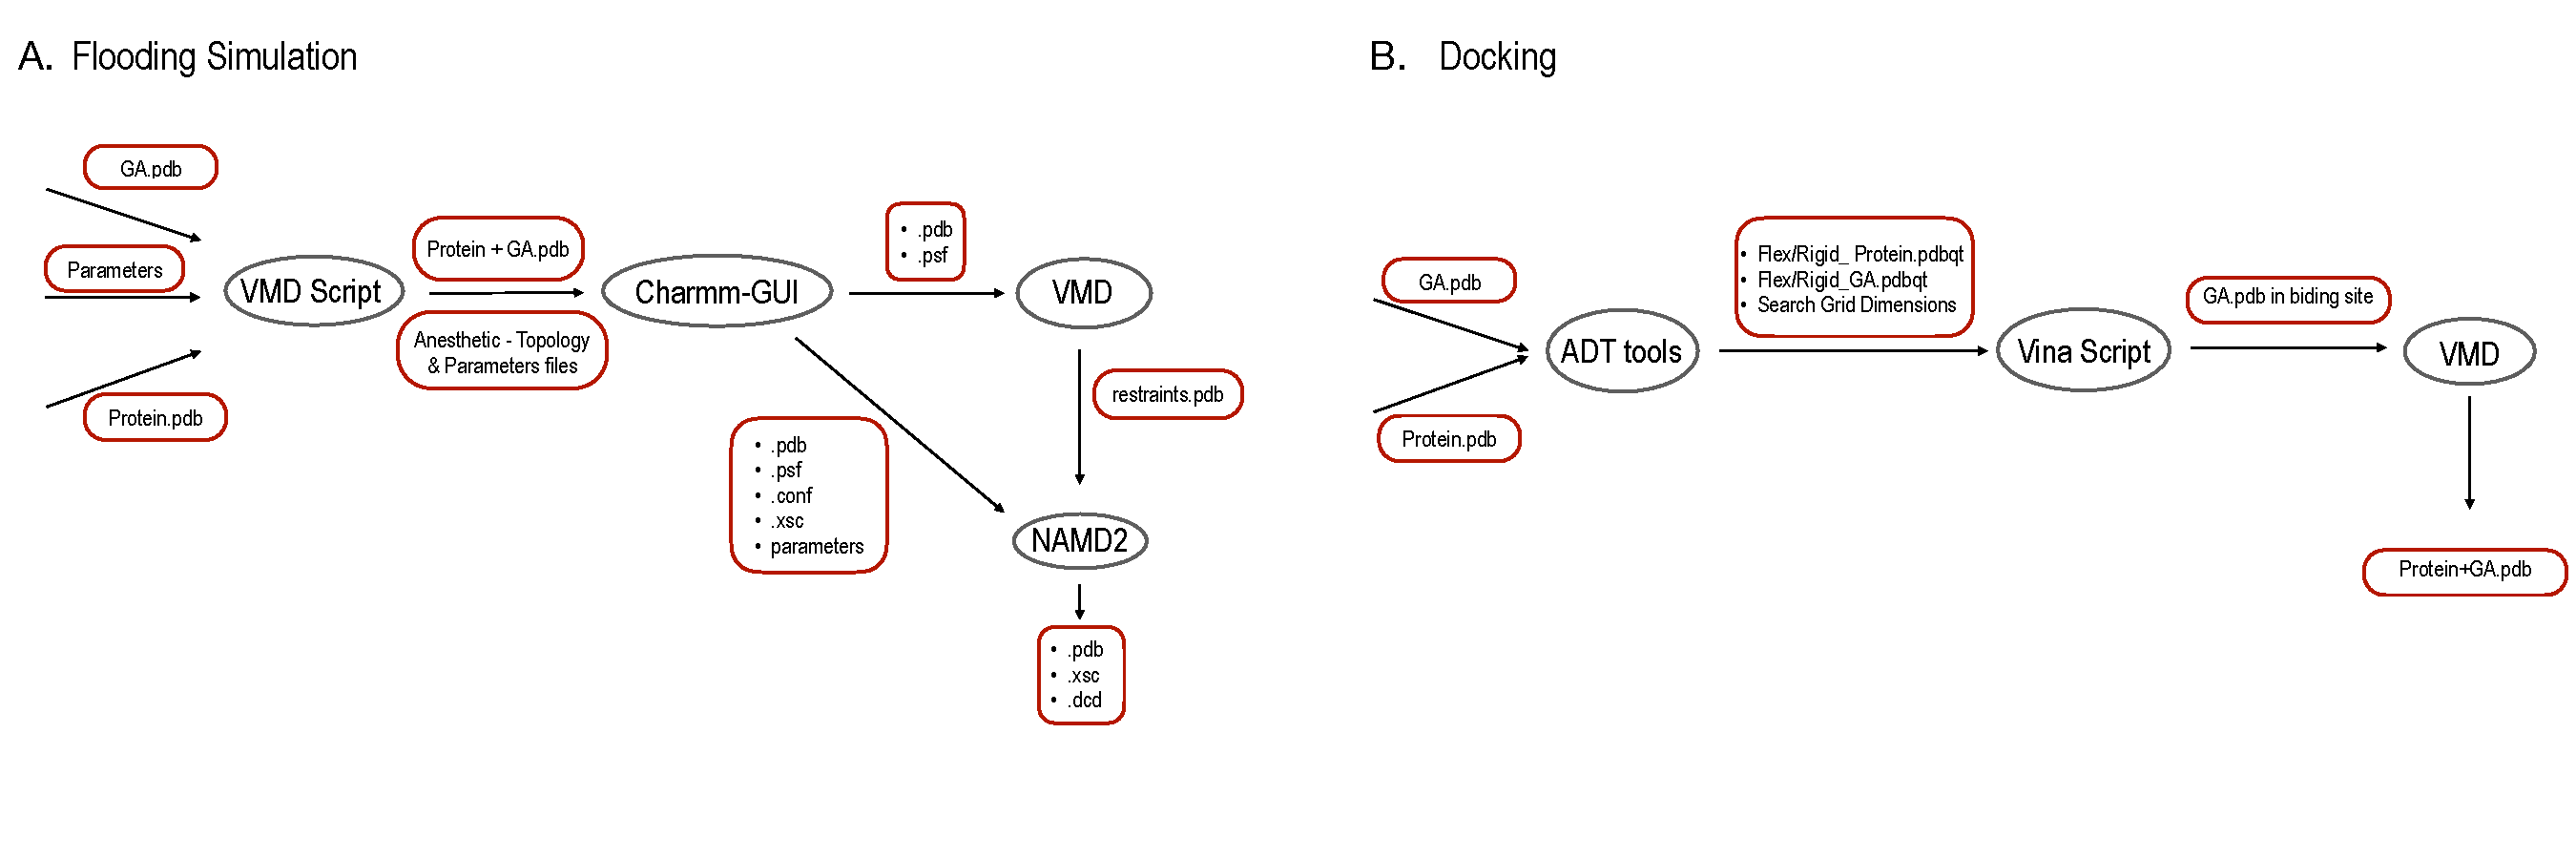
\includegraphics[width = 1\textwidth]{finlpics/Figure_1}
%\hspace{1in}
%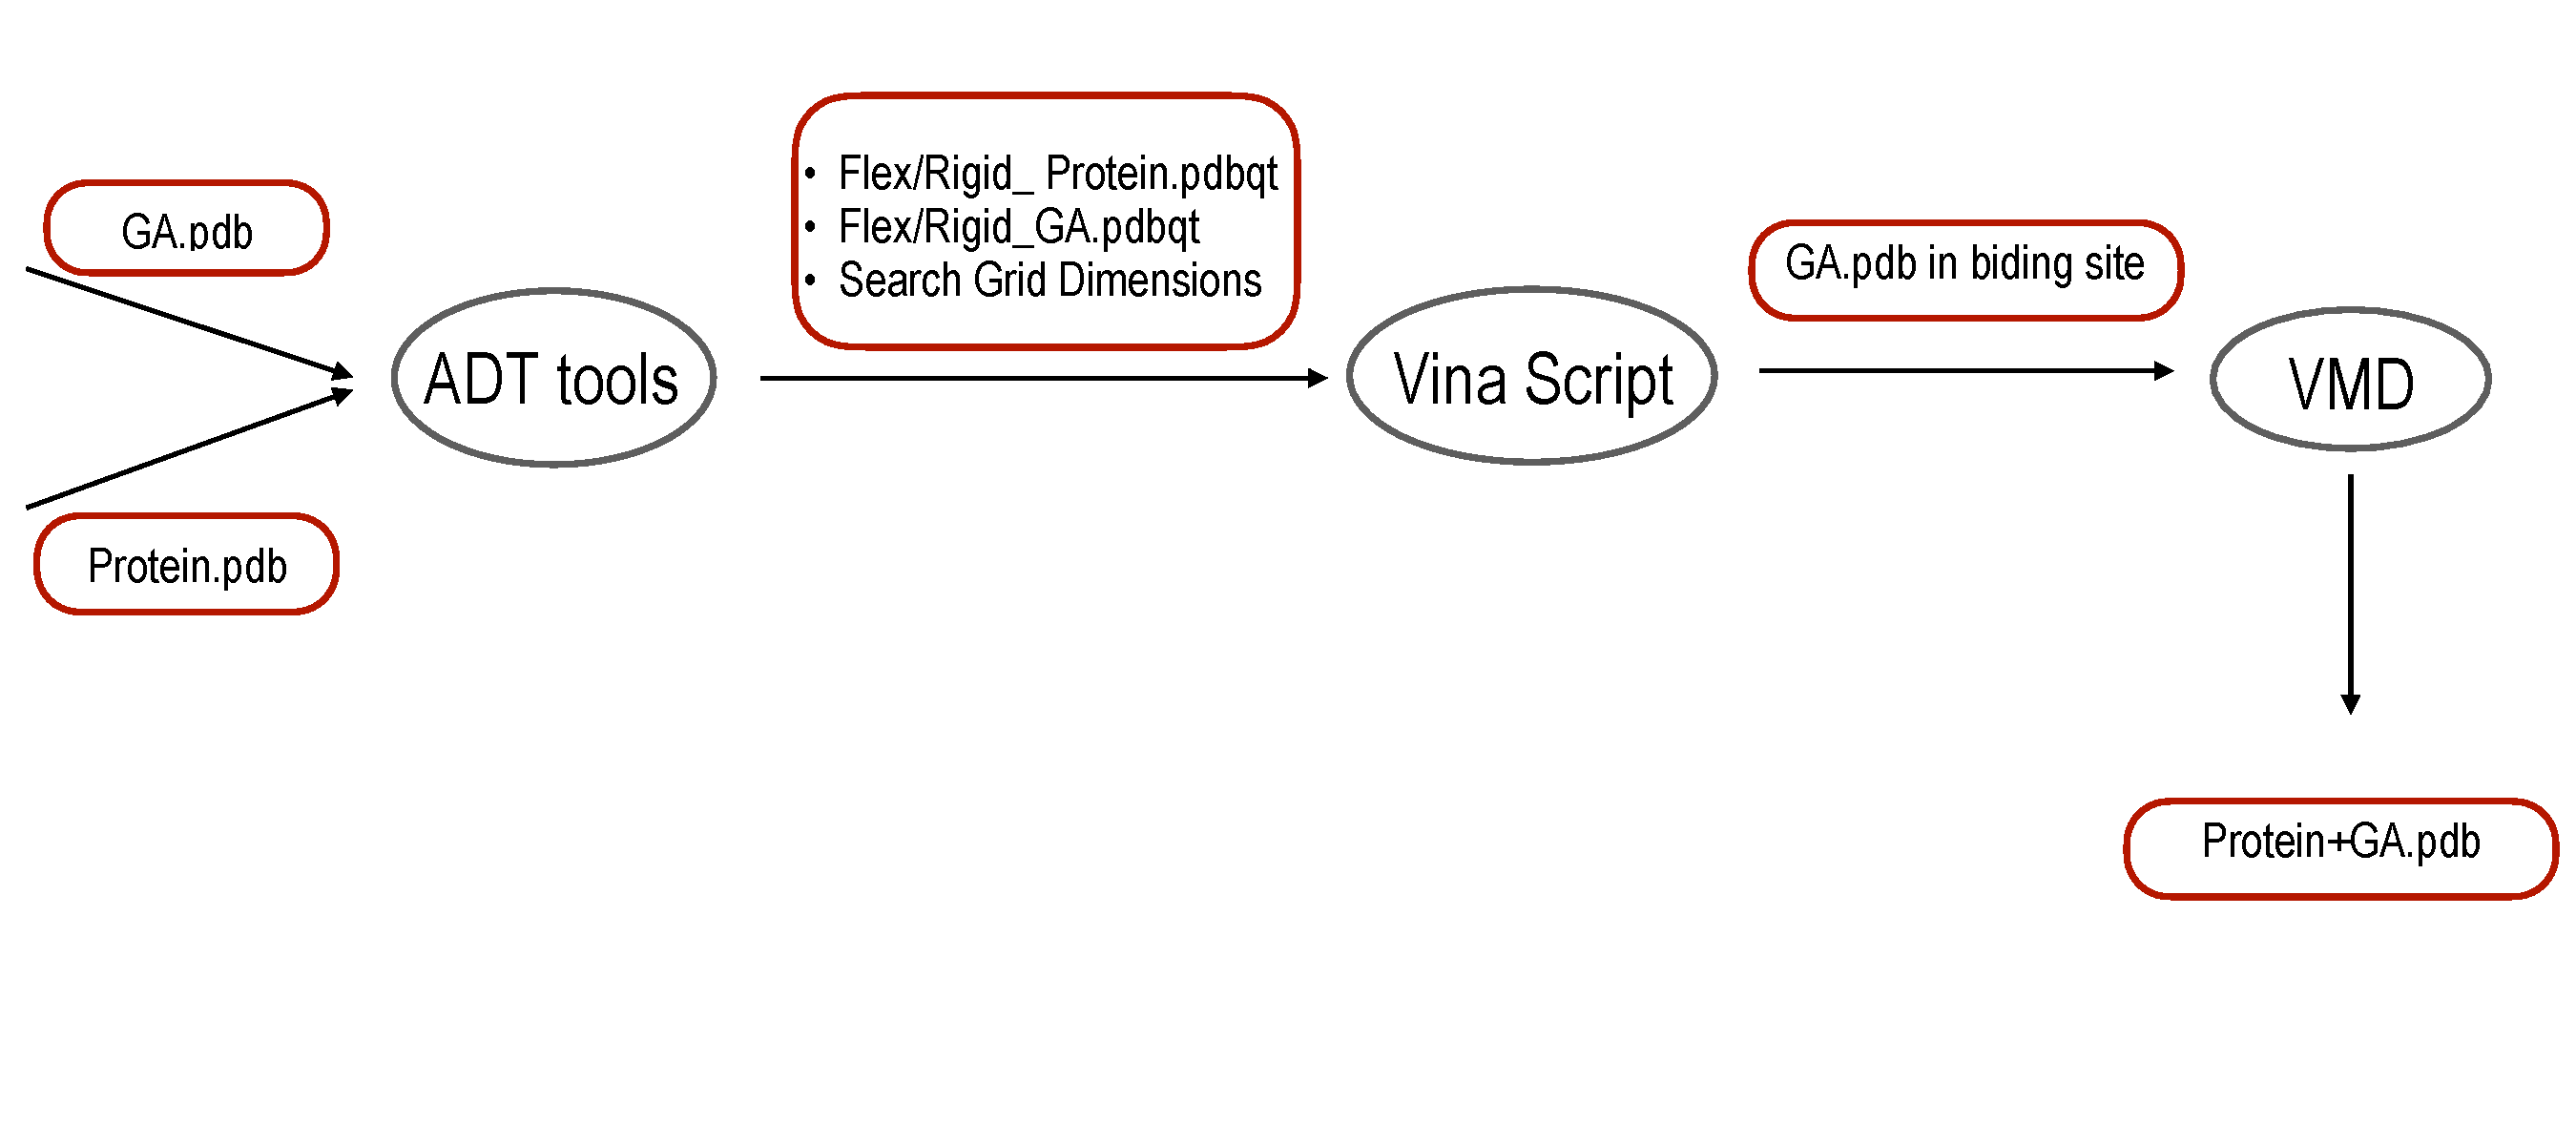
\includegraphics[width =  0.4\textwidth]{finlpics/Flowchart_docking}
\caption{Flowchart describing  the sequential steps involved in performing (left) Flooding simulation and (right) Docking using Autodock and MD simulation}
\label{fig:flowchart_flood}
\end{center}
\end{figure}

\begin{figure}
\begin{center}
\centering
%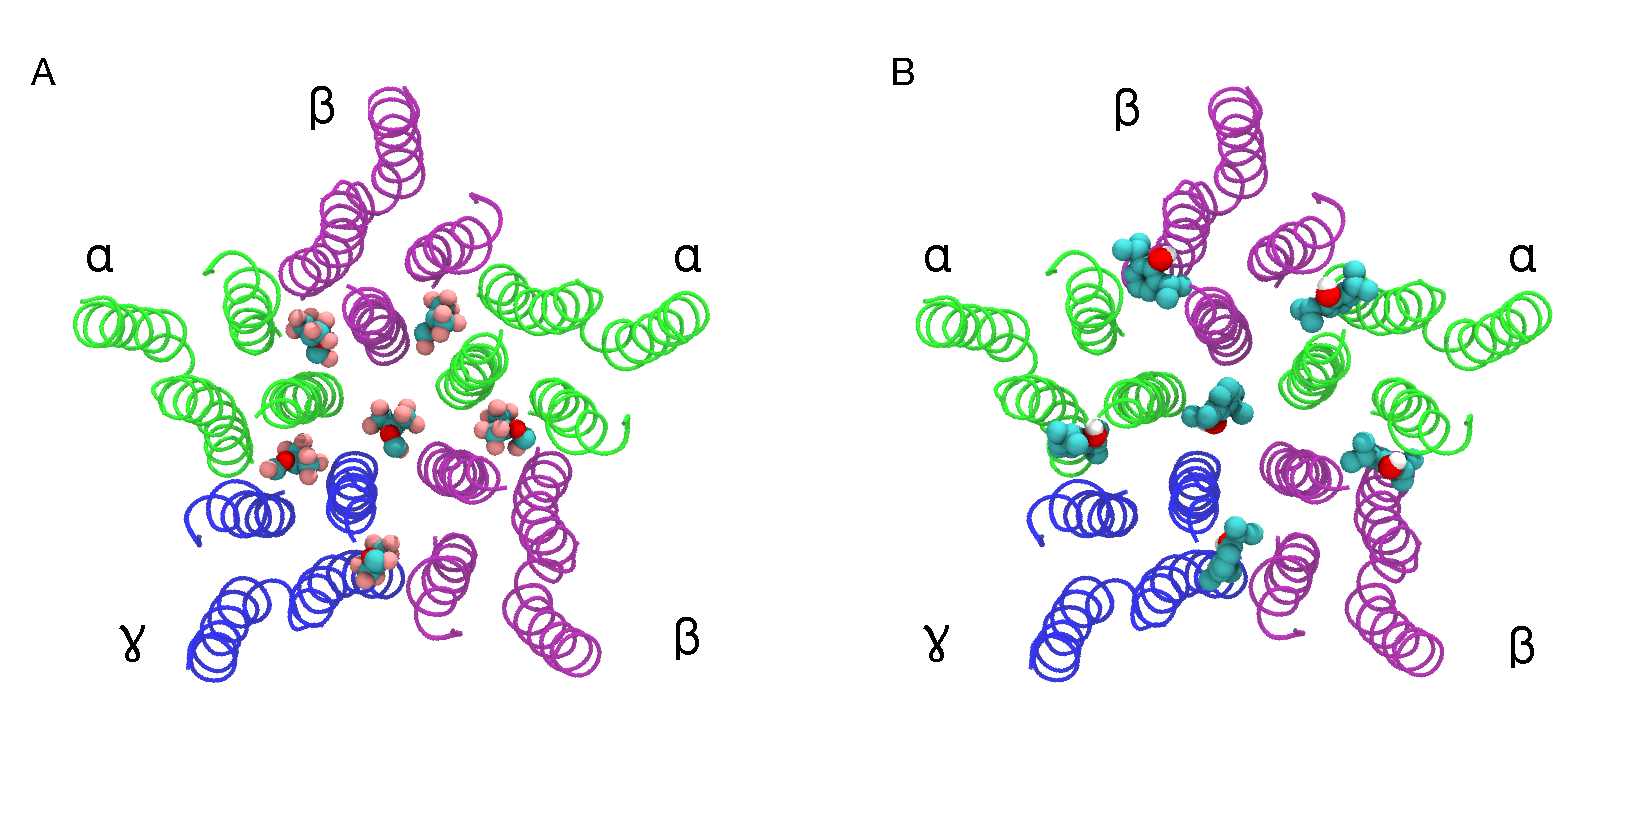
\includegraphics[width = 1\textwidth]{finlpics/dock_pic.pdf}
\caption{View of the TM domain, looking down on the membrane from the extracellular region; Sevoflurane(A) and Propofol(B) docked to the TMD of GABA(A) receptor. Docking was individually performed at all the inter-subunit sites and the pore by making few of the protein residues, flexible. For instance, at the $\alpha$-$\beta$ site, $\beta$MET289 residue side-chain was made flexible  while docking to this interface.}
\label{fig:dockPic}
\end{center}
\end{figure}


\begin{figure}
\begin{center}
\centering
%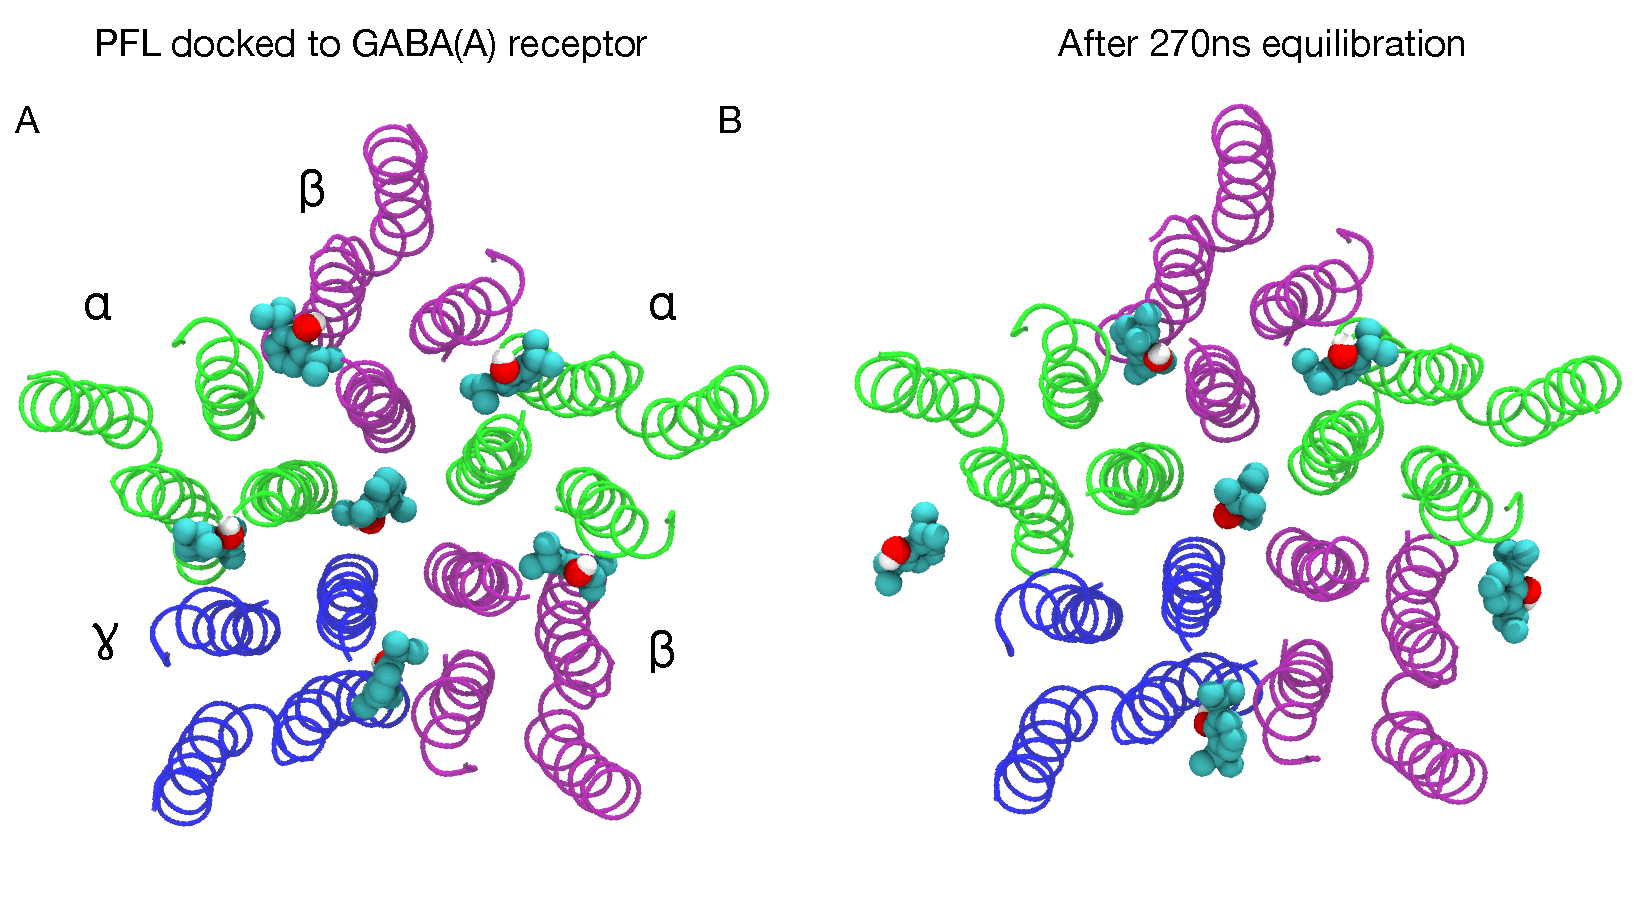
\includegraphics[width = 1\textwidth]{finlpics/PFL_equl}
\caption{View of the TM domain, looking down on the membrane from the extracellular region;   MD  of  PFL-GABA(A)  receptor  system, images depict the position of Propofol at initial and final frames of the trajectory.  Unfavorable conformation of Propofol led to expulsion of the ligand in the course of the simulation.}
\label{fig:PFLequl}
\end{center}
\end{figure}

\begin{figure}
\begin{center}
\centering
%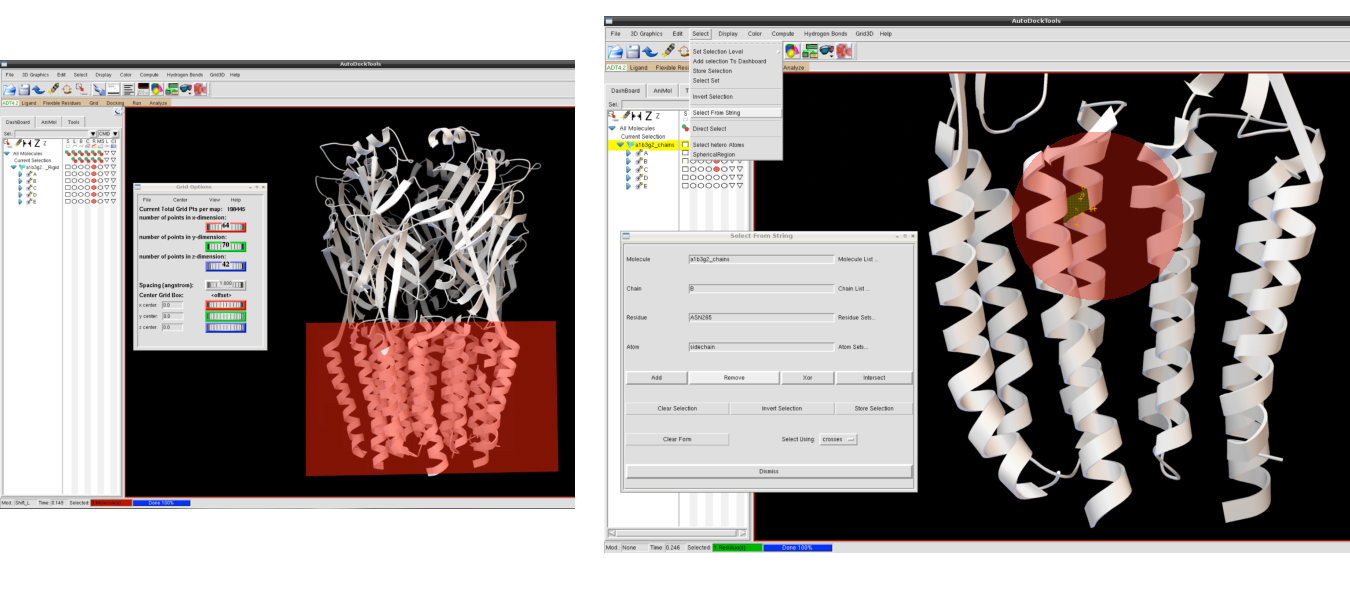
\includegraphics[width =  1\textwidth]{finlpics/adt_pic}
\caption{Screenshot of Autodock tools screen  depicting a dialogue box describing (A) the measurements of the grid box over the TMD of the protein and (B) the process of selecting the flexible residues in the protein. }
\label{fig:adtPic}
\end{center}
\end{figure}

\begin{figure}
\begin{center}
\centering
%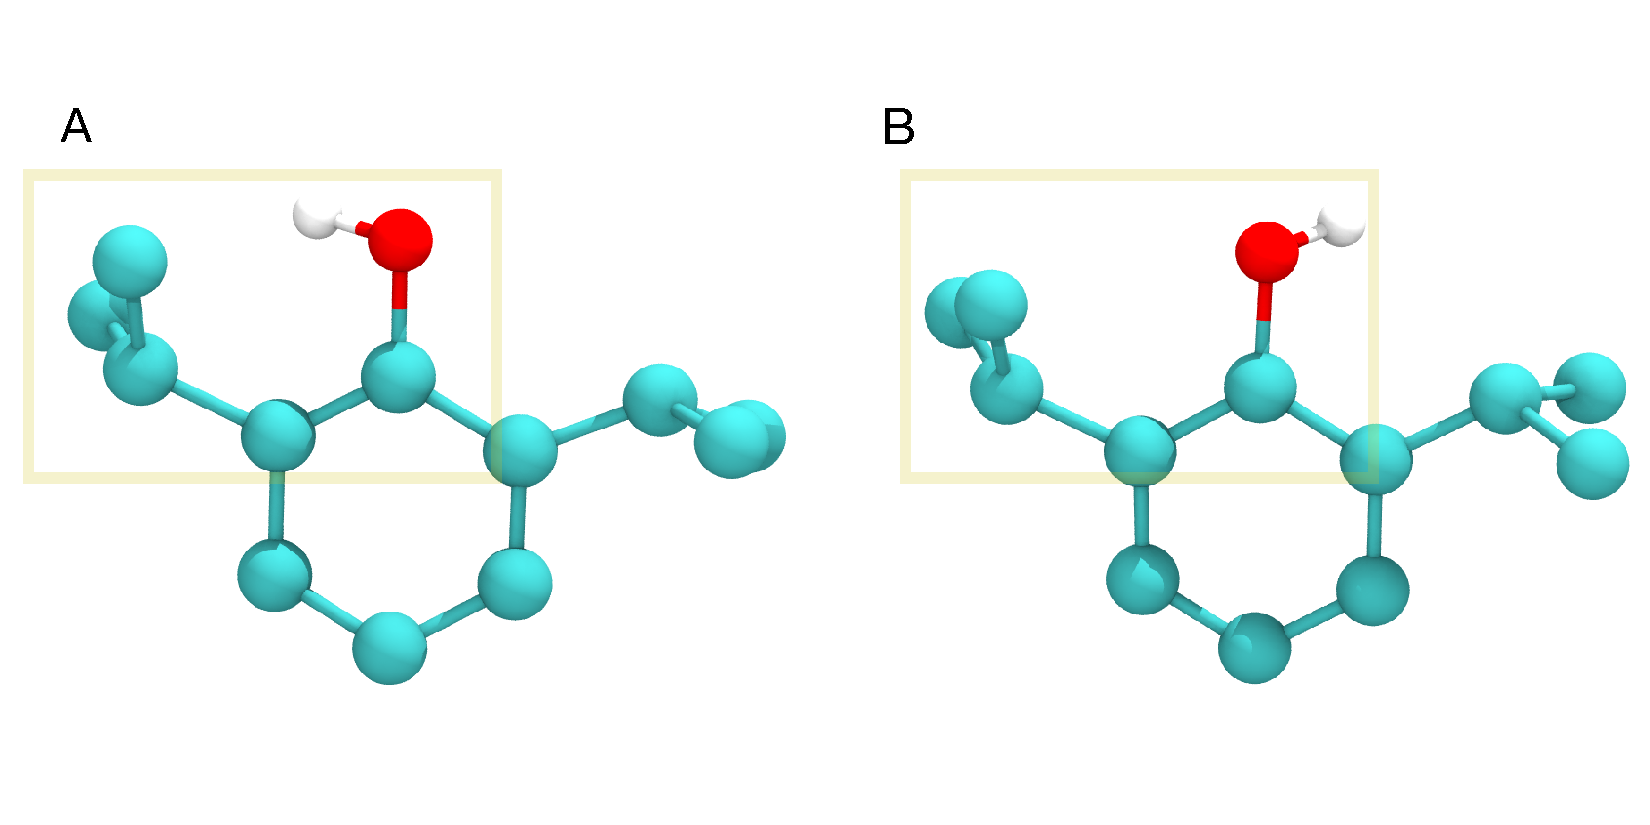
\includegraphics[width =  0.5\textwidth]{finlpics/PFL_dihed}
\caption{Comparison between an unfavorable (A) and favorable low energy (B) conformation of Propofol.}
\label{fig:PFLdihed}
\end{center}
\end{figure}

\begin{figure}
\begin{center}
\centering
%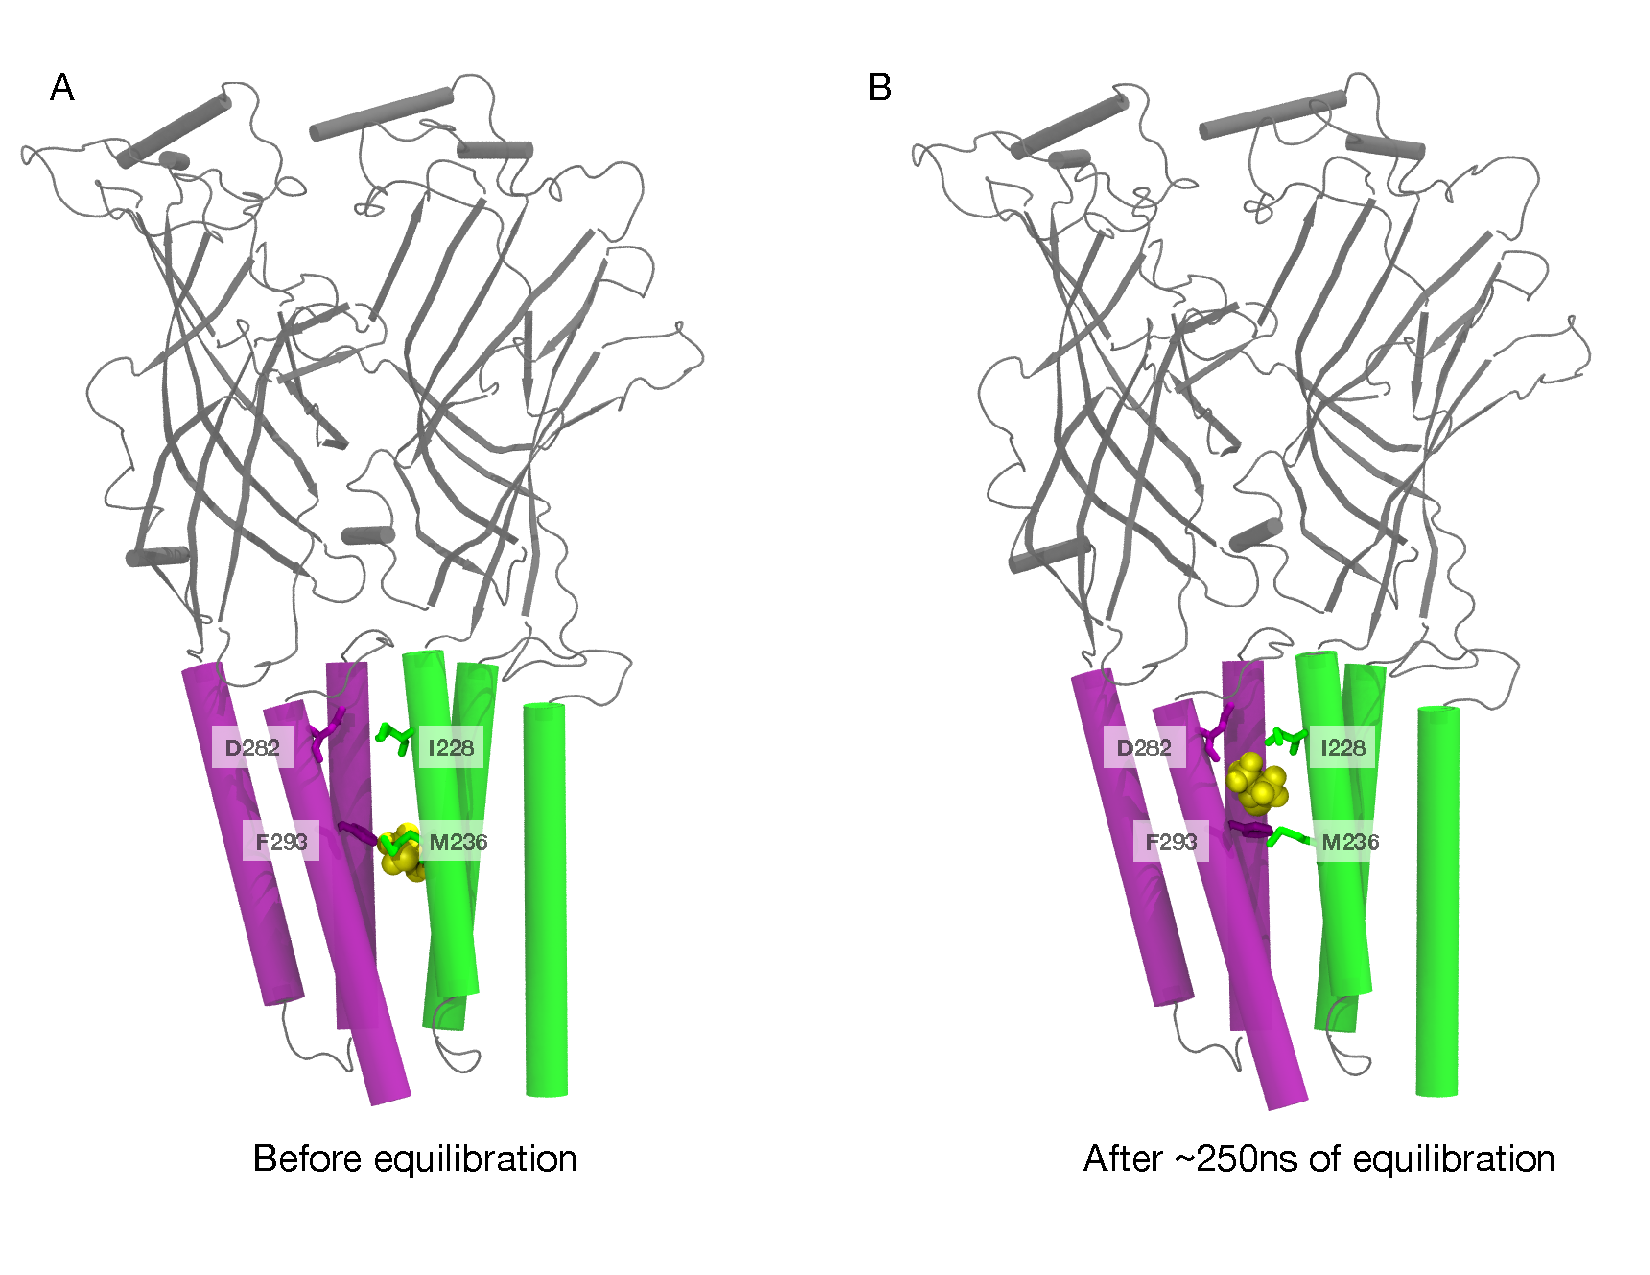
\includegraphics[width = 1\textwidth]{finlpics/sevo_MD_comp}
\caption{Side view of the sevoflurane in the $\beta$-$\alpha$ interface of the GABA(A) receptor system; Two images depicting the docked (A) and equilibrated conformation (B) of the system. Equilibration of the docked conformation allows Sevoflurane to re-orient itself at a higher affinity site.}
\label{fig:sevMD}
\end{center}
\end{figure}


\begin{figure}
\begin{center}
\centering
%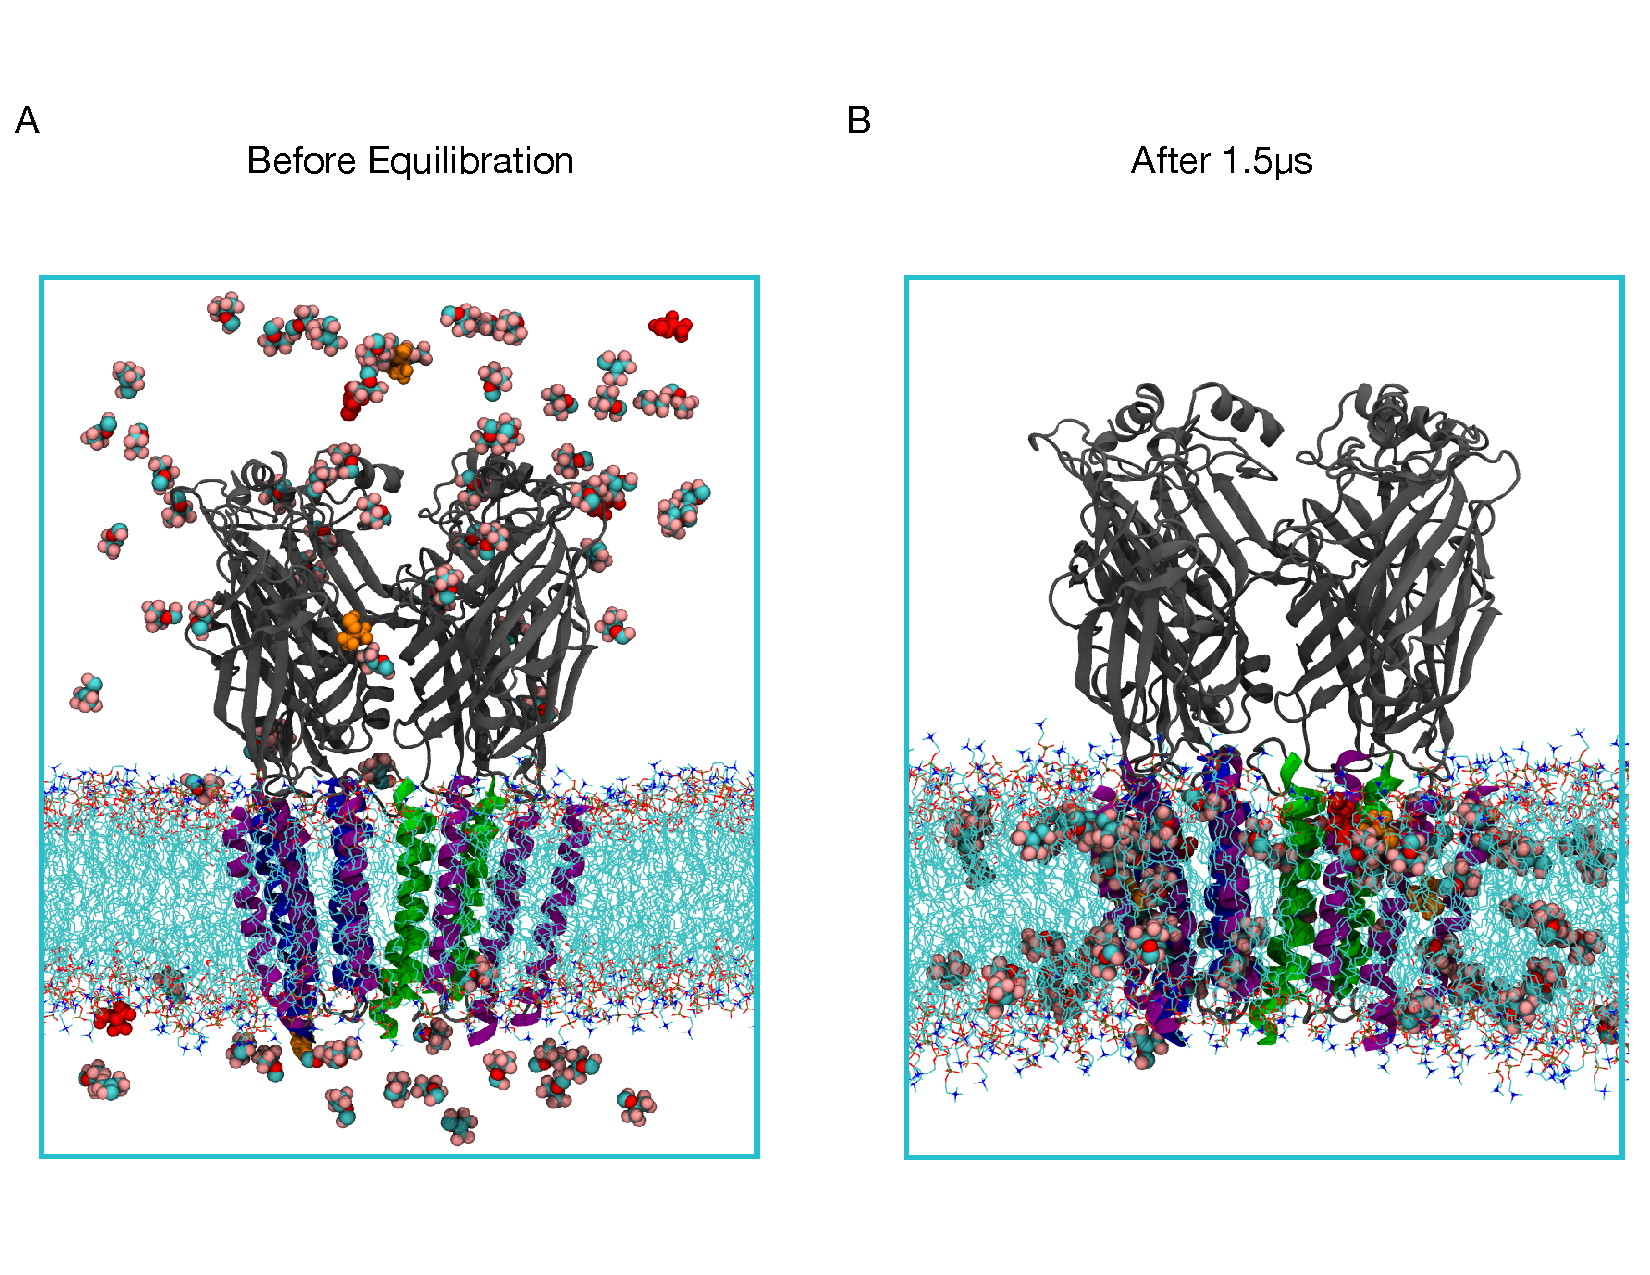
\includegraphics[width = 1\textwidth]{finlpics/sev_floodcomp}
\caption{Cross-sectional view of the Sevoflurane flooded GABA(A) receptor system with the TMD aligned along POPC lipid membrane(colored by name) and placed in a box of explicit water (molecules not shown, represented as a blue box); (A) Initial frame with Sevoflurane(colored by name) flooded in the water; After  1.5$\mu$s  Sevoflurane completely localizes in the lipid membrane with some binding the inter and intra-subunit sites(red and orange) in the TMD.}
\label{fig:sevFlood}
\end{center}
\end{figure} 

\begin{figure}
\begin{center}
\centering
%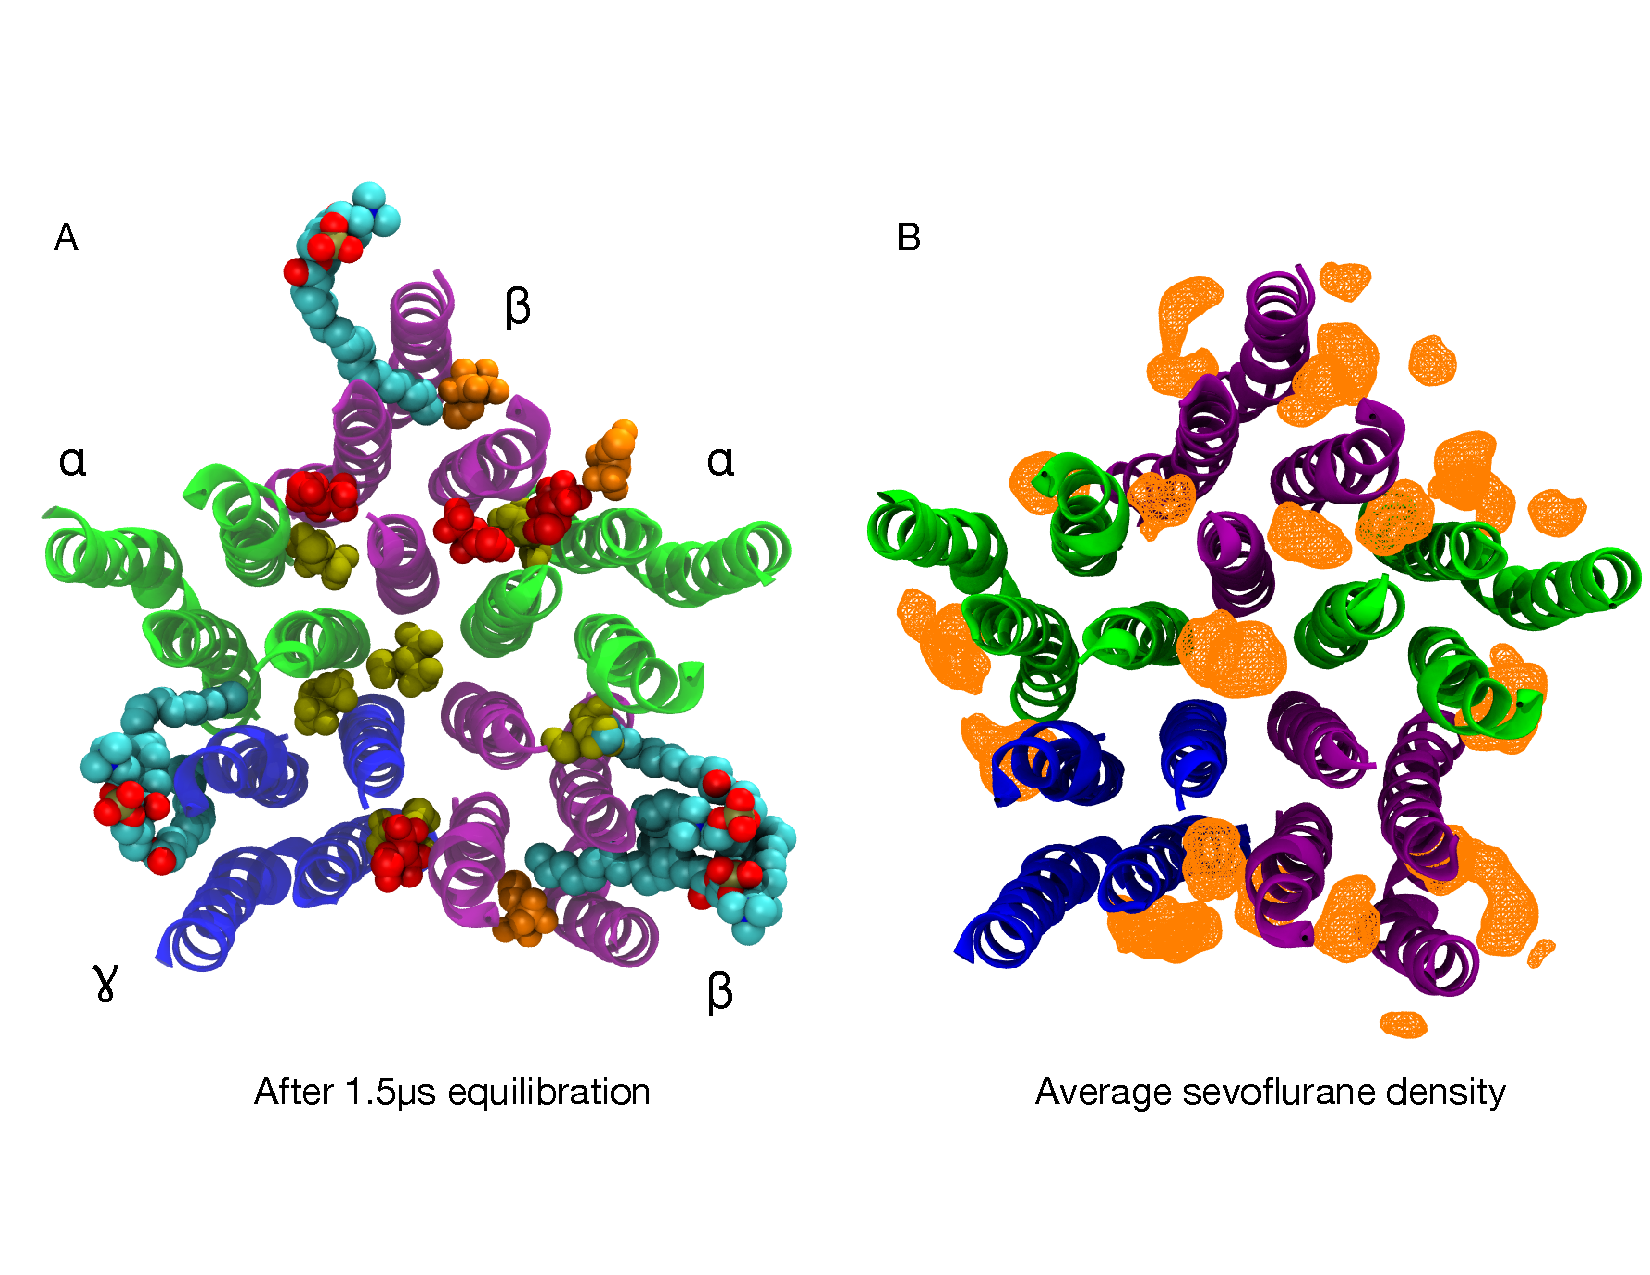
\includegraphics[width = 1\textwidth]{finlpics/sevVolMap}
\caption{View from the extracellular domain, of a Sevoflurane flooded GABA(A) receptor system; (A) Final frame from the flooding simulation  showing sevoflurane occupying the inter, intra and pore sites(Red, orange) overlaid with sevoflurane(yellow) docked using Auto-dock; Flooding simulation also identified lipid (colored by name) interference in $\beta$ intra-subunit site and and $\alpha$-$\gamma$, $\alpha$-$\beta$ intersubunit sites. (B) Image created using VMD plugin, VOL-MAP tool, to depict the density isosurface (orange)  averaged over the last 700 ns of the simulation; large mesh represent occupation over majority of the trajecotory, whereas a few smaller mesh represents occupation for lesser time.}
\label{fig:sevVolMap}
\end{center}
\end{figure}

\begin{figure}
\begin{center}
\centering
%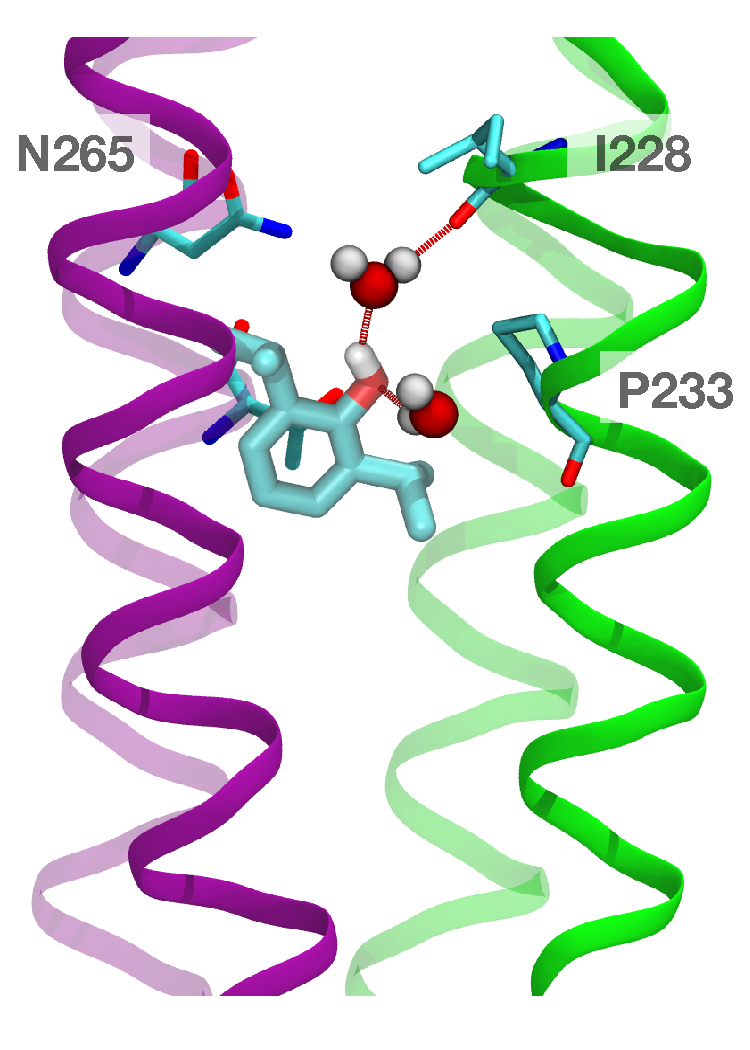
\includegraphics[width = 0.4\textwidth]{finlpics/PFL_hbonds}
\caption{Depiction of Propofol interacting with water and protein side-chains at the $\beta-$-$\alpha+$ intersubunit site, in a snapshot from a MD simulation.}
\label{fig:PFLhbond}
\end{center}
\end{figure}

\begin{figure}
\begin{center}
\centering
%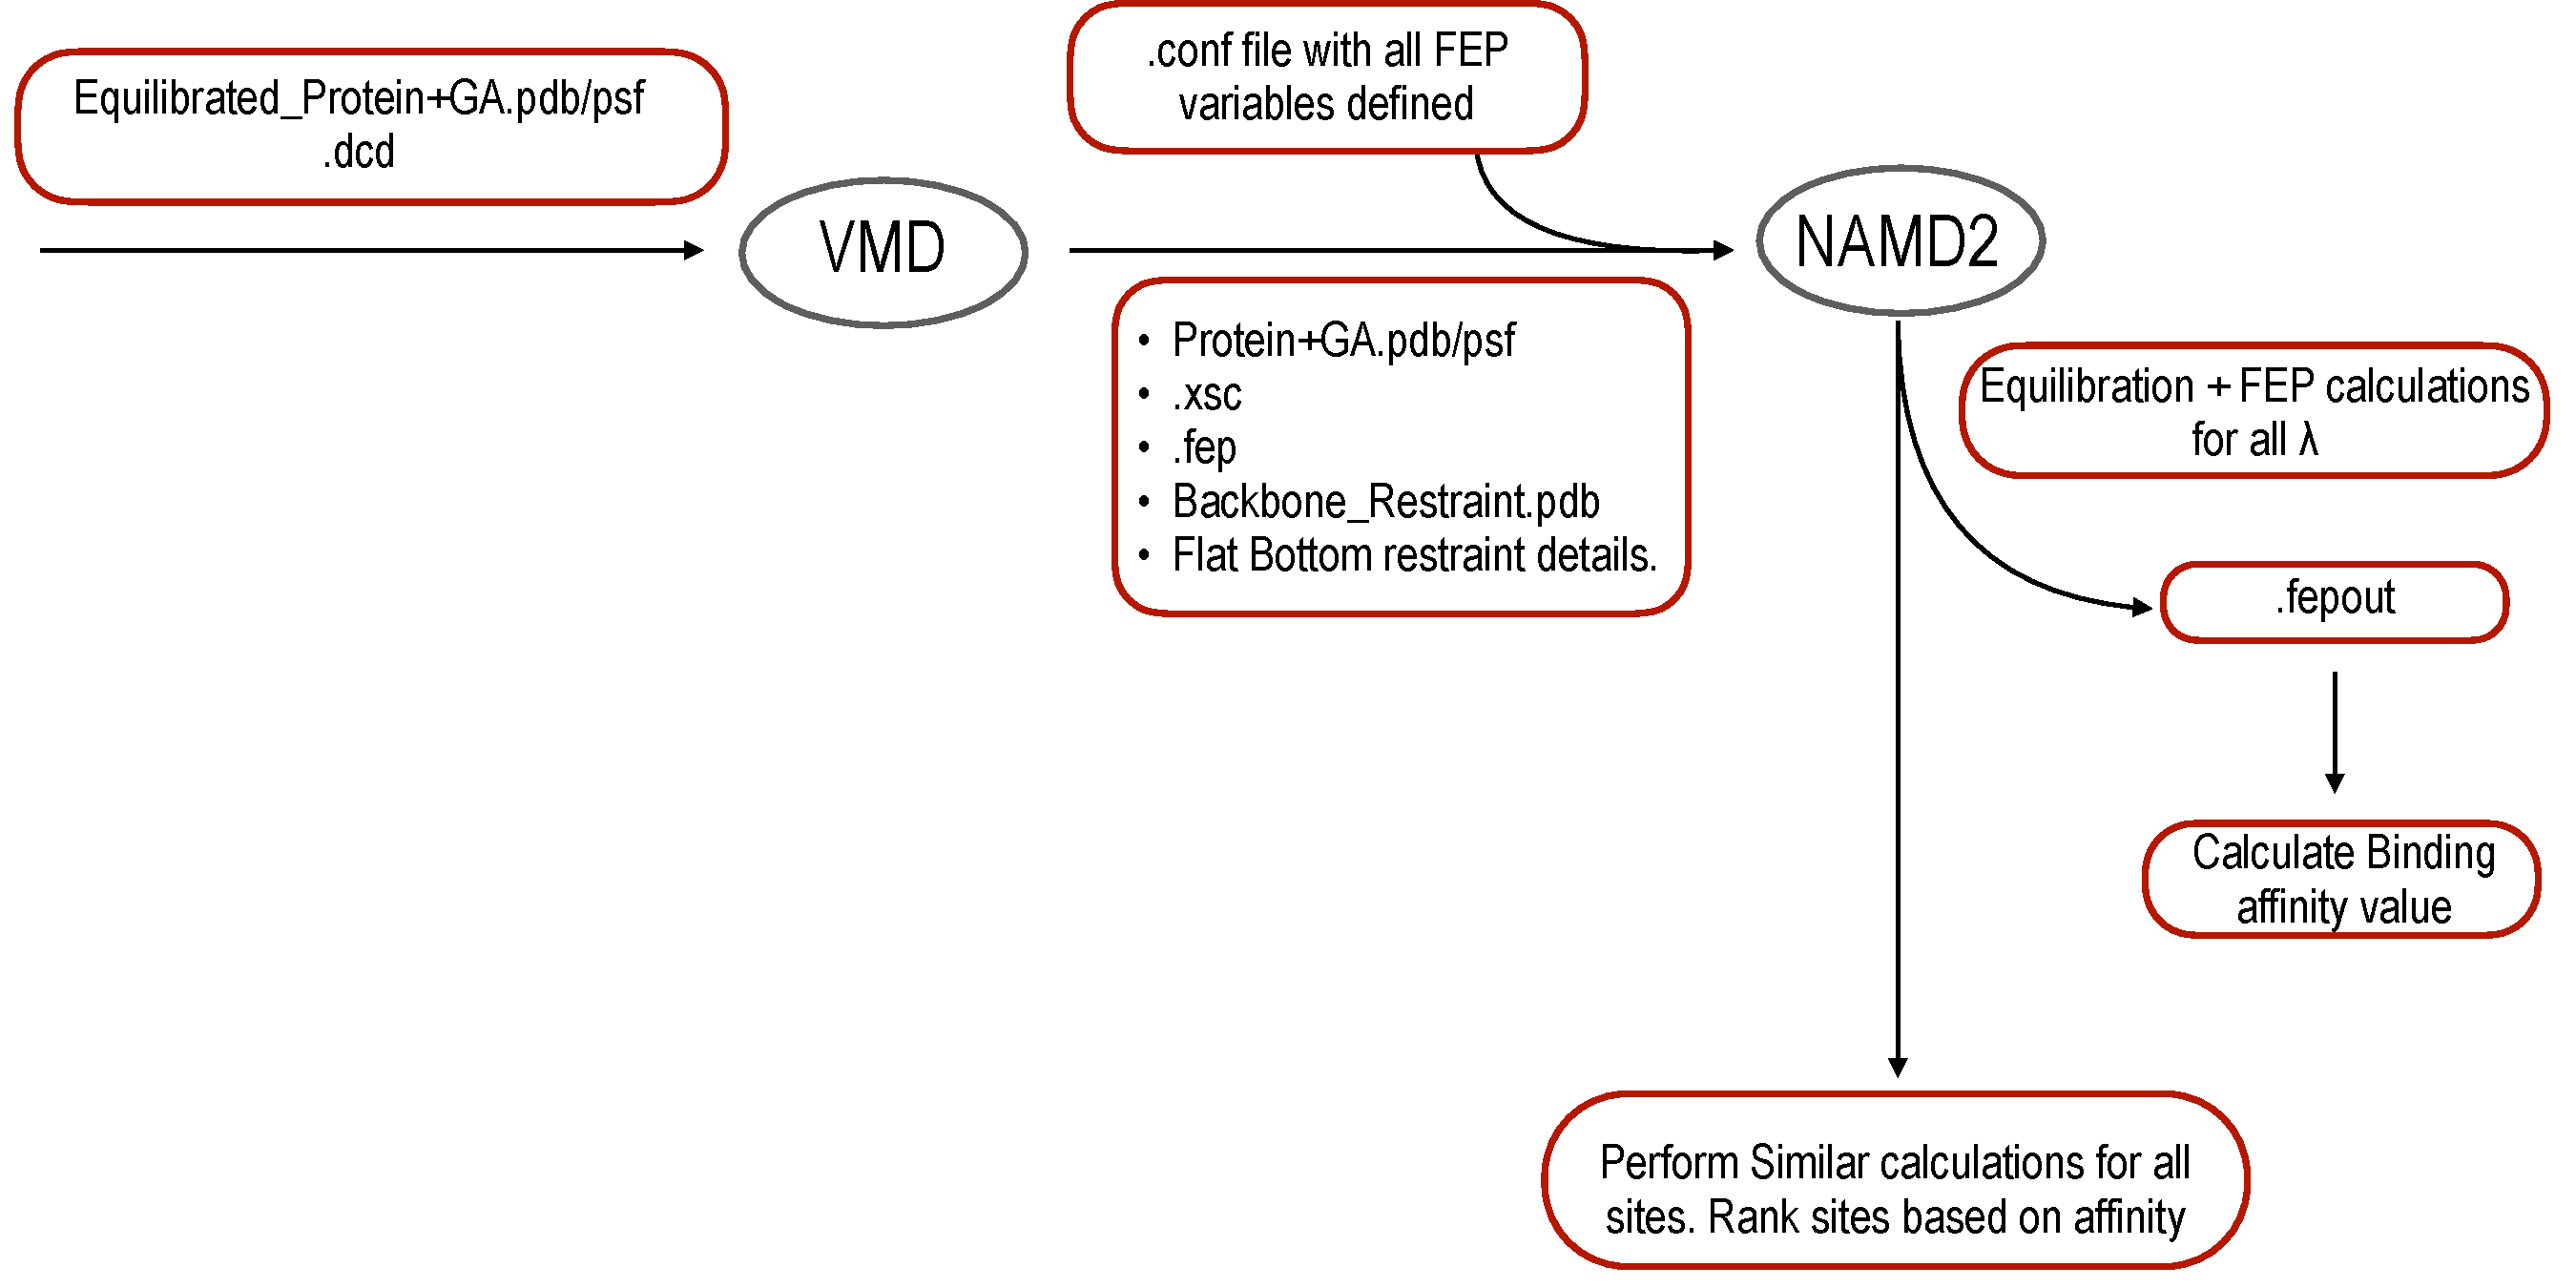
\includegraphics[width =  0.4\textwidth]{finlpics/Flowchart_FEP}
\caption{Flowchart describing  the sequential steps involved in calculating binding affinity of anesthetics}
\label{fig:flowchart_FEP}
\end{center}
\end{figure}

\begin{figure}
\begin{center}
\centering
%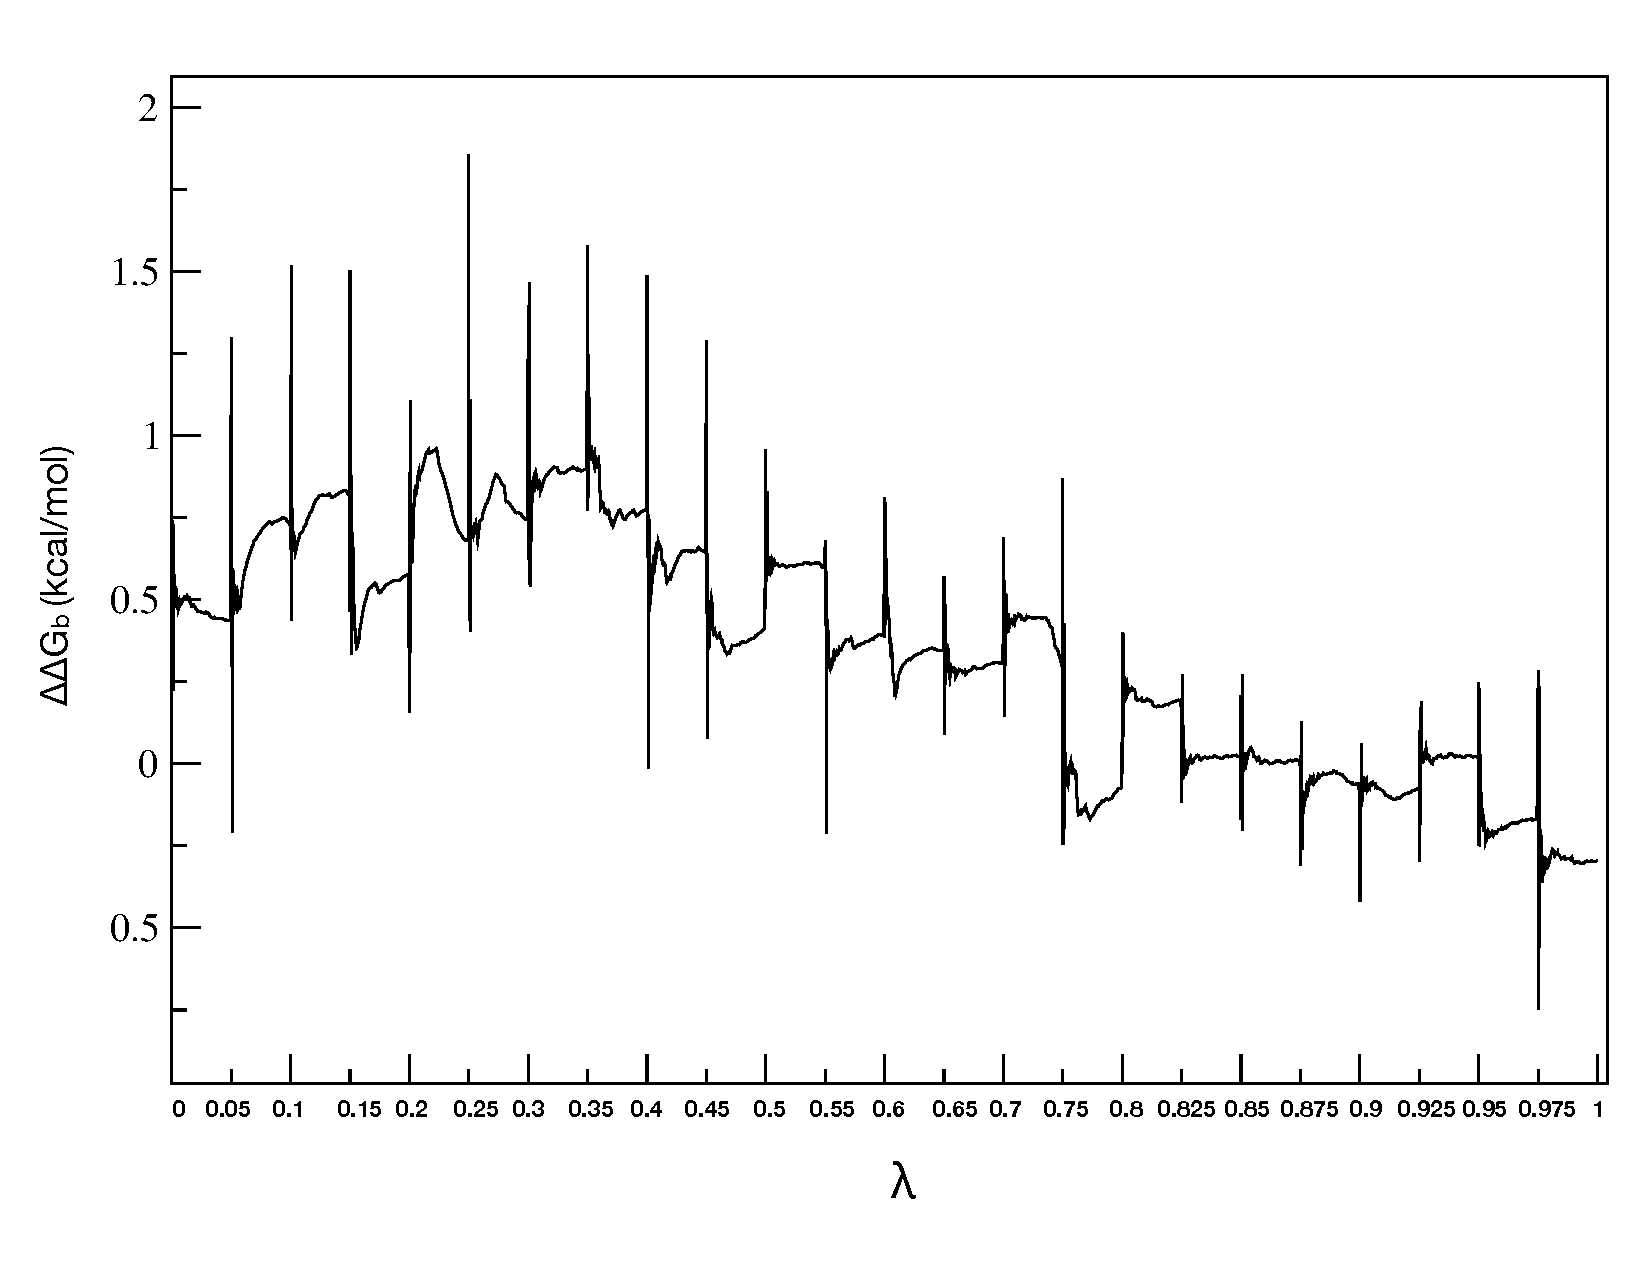
\includegraphics[width =  0.75\textwidth]{finlpics/per_lambda}
\caption{Sample data set for $\Delta\Delta G_{i}$ variations per window.% for decoupling sevoflurane from an intersubunit site in GABA(A) receptor. 
Curves that plateau (as at $\lambda = 0.825$ to 0.85) indicate convergence, while curves that still change rapidly by the end of the window (as at $\lambda = 0.20$ to 0.25) indicate a need for extending the calculation for that window or dividing the window into two.  }
\label{fig:lambda}
\end{center}
\end{figure}


\end{document}